%input macros (i.e. write your own macros file called MacroFile1.tex)
%\newcommand{\PdfPsText}[2]{
  \ifpdf
     #1
  \else
     #2
  \fi
}

\newcommand{\IncludeGraphicsH}[3]{
  \PdfPsText{\includegraphics[height=#2]{#1}}{\includegraphics[bb = #3, height=#2]{#1}}
}

\newcommand{\IncludeGraphicsW}[3]{
  \PdfPsText{\includegraphics[width=#2]{#1}}{\includegraphics[bb = #3, width=#2]{#1}}
}

\newcommand{\InsertFig}[3]{
  \begin{figure}[!htbp]
    \begin{center}
      \leavevmode
      #1
      \caption{#2}
      \label{#3}
    \end{center}
  \end{figure}
}


%%% Local Variables: 
%%% mode: latex
%%% TeX-master: "~/Documents/LaTeX/CUEDThesisPSnPDF/thesis"
%%% End: 


\documentclass[oneside,12pt]{Classes/CUEDthesisPSnPDF}

\ifpdf
    \pdfinfo { /Title  (The Poetry Pioneer)
               /Creator (TeX)
               /Producer (pdfTeX)
               /Subject (Poetic Precision)
               /Keywords (PhD, Thesis)}
    \pdfcatalog { /PageMode (/UseOutlines)
                  /OpenAction (fitbh)  }
\fi

\title{The Poetry Pioneer}

\ifpdf
  \author{\href{mailto:nbn10@doc.ic.ac.uk}{Nitin Nihalani}}
  \collegeordept{\href{http://www.doc.ic.ac.uk}{Department of Computing}}
  \university{\href{http://www.ic.ac.uk}{Imperial College London}}
% insert below the file name that contains the crest in-place of 'UnivShield'
  \crest{
\includegraphics[width=70mm]{UnivShield}}
  \crest{
\includegraphics[width=70mm]{logo}}
\else
  \author{Nitin Nihalani}
  \collegeordept{Department of Engineering}
  \university{Imperial College London}
% insert below the file name that contains the crest in-place of 'UnivShield'
  \crest{
\includegraphics{UnivShield}}
  \crest{
\includegraphics[bb = 0 0 292 336, width=70mm]{logo}}
\fi
%
% insert below the file name that contains the crest in-place of 'UnivShield'
% \crest{\IncludeGraphicsW{UnivShield}{40mm}{14 14 73 81}}
%
\renewcommand{\submittedtext}{An interim report for}
\degree{MEng Computing (AI)}
\degreedate{Individual Project}

% turn of those nasty overfull and underfull hboxes
\hbadness=10000
\hfuzz=50pt

% Put all the style files you want in the directory StyleFiles and usepackage like this:
\usepackage{StyleFiles/watermark}
\usepackage{cleveref}

% Comment out the next line to get single spacing
\onehalfspacing

\usepackage{titlesec}
\titlespacing*{\chapter}{0pt}{-60pt}{20pt}
\titleformat{\chapter}[display]{\normalfont\huge\bfseries}{\chaptertitlename\ \thechapter}{20pt}{\Huge}
\usepackage{multicol}
%\usepackage{cite}
\usepackage[utf8]{inputenc}
\usepackage{listings}
\usepackage{algorithmicx}
\usepackage{algpseudocode}
\usepackage{algorithm}
\usepackage{color}
\usepackage{caption}
\usepackage{subcaption}
\usepackage{tikz}
\usetikzlibrary{arrows}
\usetikzlibrary{trees}
\lstset{frame=tb,
  language=Python,
  aboveskip=3mm,
  belowskip=3mm,
  showstringspaces=false,
  columns=flexible,
  basicstyle={\small\ttfamily},
  numbers=none,
  breaklines=true,
  breakatwhitespace=true
  tabsize=2
}

\addbibresource{References/poetry_references.bib}
\nocite{*}

\begin{document}

%\language{english}

% A page with the abstract on including title and author etc may be
% required to be handed in separately. If this is not so, then comment
% the below 3 lines (between '\begin{abstractseparte}' and 
% 'end{abstractseparate}'), normally like a declaration ... needs some more
% work, mind as environment abstracts creates a new page!
% \begin{abstractseparate}
%   %%% Thesis Abstract --------------------------------------------------
\chapter{Abstract}
\ifpdf
    \graphicspath{{Abstract/AbstractFigs/PNG/}{Abstract/AbstractFigs/PDF/}{Abstract/AbstractFigs/}}
\else
    \graphicspath{{Abstract/AbstractFigs/EPS/}{Abstract/AbstractFigs/}}
\fi




% ----------------------------------------------------------------------


%%% Local Variables: 
%%% mode: latex
%%% TeX-master: "../thesis"
%%% End: 

% \end{abstractseparate}




% Using the watermark package which is in StyleFiles/
% and to remove DRAFT COPY ONLY appearing on the top of all pages comment out below line
%\watermark{DRAFT COPY ONLY}


\maketitle
\parindent 0pt


%set the number of sectioning levels that get number and appear in the contents
\setcounter{secnumdepth}{4}
\setcounter{tocdepth}{4}

\frontmatter % book mode only
\pagenumbering{roman}
%\include{Dedication/dedication}
%% Thesis Acknowledgements ------------------------------------------------


%\begin{acknowledgementslong} %uncommenting this line, gives a different acknowledgements heading
\begin{acknowledgements}      %this creates the heading for the acknowlegments





\end{acknowledgements}
%\end{acknowledgmentslong}

% ------------------------------------------------------------------------

%%% Local Variables: 
%%% mode: latex
%%% TeX-master: "../thesis"
%%% End: 


\tableofcontents
%\listoffigures
%\addcontentsline{toc}{chapter}{nomenclature}

\mainmatter % book mode only
%%% Thesis Abstract --------------------------------------------------
\chapter{Abstract}
\ifpdf
    \graphicspath{{Abstract/AbstractFigs/PNG/}{Abstract/AbstractFigs/PDF/}{Abstract/AbstractFigs/}}
\else
    \graphicspath{{Abstract/AbstractFigs/EPS/}{Abstract/AbstractFigs/}}
\fi




% ----------------------------------------------------------------------


%%% Local Variables: 
%%% mode: latex
%%% TeX-master: "../thesis"
%%% End: 


\parskip 6pt

%%% Thesis Introduction --------------------------------------------------
\chapter{Introduction}
\ifpdf
    \graphicspath{{Introduction/IntroductionFigs/PNG/}{Introduction/IntroductionFigs/PDF/}{Introduction/IntroductionFigs/}}
\else
    \graphicspath{{Introduction/IntroductionFigs/EPS/}{Introduction/IntroductionFigs/}}
\fi
\emph{"Dream in a pragmatic way." - Aldous Huxley}
\section{Motivation}

Computational Semantics is a relatively young and fashionable topic in Computational Linguistics. It involves finding representations and algorithms that are able to cope with the \textit{meaning} of linguistic utterances.

Pragmatics is an even younger discipline, concentrating on the context of those utterances. When we as humans read or listen to any linguistic output, we build a representation of the objects, people, actions, descriptions, relationships and anything else to provide context to the experience. For example, the phrase \textit{"I have a green light"} may mean that I have been granted permission for something, or that I literally have a lamp with a green tint. 

Indeed a similar approach is taken when writing or speaking - one has a purpose and a message that would like to be passed and the language used helps to build such context. For example, if I aim to tell you that I have a lot of work, I could simply say that or say I am 'drowning' in work. The latter helps you, the reader, realise that not only do I have a lot of work but that I also cannot handle it.

For a computer to truly converse in a manner indistinguishable to humans, as is the aim of the elusive Turing Test, it must be able to handle pragmatics along with syntax and semantics. This requires a deep understanding of words not as a linguistic unit, but as the objects, actions and descriptions they represent. They should then be used with a purpose when generating text, as human writers and speakers do.

Poetry is a linguistic art form designed to help convey a particular, well-defined message in a memorable and powerful way. Poets write poems that are succinct in length but dense in meaning by employing a number of techniques, such as rhyme and rhythm. 

Different types of poetry each have their own sets of constraints, features and priorities that define their best usage. For example, narrative poems convey characters, relationships and actions while descriptive ones are used to give a comprehensive linguistic illustration. Furthermore, rhythm and rhyme can be used to provide melody making it pleasant to hear and applicable to songs, but alliteration can be used to create suspense and a sense of danger.

In this paper, we use poetry as the catalyst with which to develop computational semantics and pragmatics. We aim to create a system that can analyse poetry and build a contextual representation of it, as well as generate poetry with an underlying purpose and message.

The proposed implementation comes in three phases:
\begin{enumerate}
\item{First we will write the analysis module, which detects a wide range of poetic features in a single poem. It also aims to represent the context of the poem with Discourse Representation Structures (DRSs), outlined in section \ref{sec:drt}.}

\item{Then we run many poems of the same type through the analysis module and then abstract away the common features between the given poems. This includes a general structure for the DRSs of that class of poem.}

\item{Finally we generate poems with a purpose as guided by the structure of the DRS. We will also utilise third-party libraries to build semantically and syntactically valid lines of poetry that also use poetic features. Poeticness and creativity is prioritised in the selection of words and phrases during the generation process. A dry run of this phase is given in the appendix.}
\end{enumerate}



%-----------------------------------

\section{Objectives}
The overarching primary objective of this system is \textit{pragmatic competence}. We aim to generate poetry that demonstrates some understanding of context with regards to descriptions, actions and relationships of people and objects, and with careful text and sentence planning for that context.

Thereafter, we wish to create a system that:
\begin{itemize}
\item{identifies a broad list of features in a single poem.} 
\item{abstracts features of a given class of poems or texts that have been analysed.}
\item{learns the features of a wide variety of different classes of poems.}
\item{produces poems, given natural language 'seeds' of inspiration, that are:}
	\begin{itemize}
	\setlength{\itemsep}{0pt}
	\item{novel,}
	\item{syntactically valid,}
	\item{semantically interpretable,}
	\item{pragmatically comprehensible,}
	\item{evident of a set of desired features.}
	\end{itemize} 
\item{is able to digress slightly from learned features in its use of poetic techniques in search of creativity.}
\end{itemize}

%---------------------------------------------------

\section{Contributions}
This project makes contributions towards both Computational Creativity and Computational Linguistics.
\begin{itemize}
\item{We demonstrate the ability for computer systems to assess written natural language works in terms of its structure, common words and phrases, rhetoric and poetic features such as rhyme, rhythm and alliteration.}
\item{We will investigate the appropriateness of Discourse Representation Theory (DRT) as a semantic representation of poetry from which we can derive pragmatics in terms of characters, objects and locations, descriptions of them, relationships between them and the actions that they executed.}
\item {We demonstrate the ability to abstract common written features out of a large number of comparable texts.}
\item{We take in a step in the direction of using the web as a source of material and conceptual inspiration for creative acts.}
\item{We demonstrate Discourse Representation Theory as an effective tool for guiding the macro- and micro- planning stages of natural language generation.}
\item{We demonstrate the effectiveness of third-party libraries for the surface realisation stage of Natural Language Generation.}
\item{We provide a tool for poetry creation from natural language seeds of inspiration.}
\item{We investigate the applicability of the new FACE and IDEA descriptive models for evaluation.}
\end{itemize}


%%% ----------------------------------------------------------------------

%%% Local Variables: 
%%% mode: latex
%%% TeX-master: "../thesis"
%%% End: 

% \pagebreak[4]
% \hspace*{1cm}
% \pagebreak[4]
% \hspace*{1cm}
% \pagebreak[4]

\chapter{Background}
\ifpdf
    \graphicspath{{Design/DesignFigs/PNG/}{Design/DesignFigs/PDF/}{Design/DesignFigs/}}
\else
    \graphicspath{{Design/DesignFigs/EPS/}{Design/DesignFigs/}}
\fi

This chapter gives a brief overview of the features and classes of poetry that exist, along with why people are interested in writing them. We will discuss, critique and gather inspiration from the related work in the area of poetry generation that most relate to the approach taken in this paper. We then give brief overviews into the fields of Computational Linguistics and Computational Creativity, both of which are involved in the task of automatic poetry generation. These overviews are by no means complete or comprehensive, but should provide enough information for those not familiar with the areas to understand and appreciate this paper.

\section{Poetry Theory}

To fully comprehend the task that we are about to undertake, we need to have an understanding of poetry as an art form. It is ever-evolving and different styles have emerged over the years. Here we discuss those styles and the underlying reason for why poetry is written.

\subsection{The Purpose of Poetry}
\label{sec:purpose}
Merriam-Webster dictionary defines poetry as:\\
\emph{'writing that formulates a concentrated imaginative awareness of experience in language chosen and arranged to create a specific emotional response through meaning, sound, and rhythm.'}

Let us break this down:
\begin{itemize}
\item{\textit{\textbf{Formulates}} implies that there is method to the process of writing a poem.}
\item{\textit{\textbf{Concentrated}} accentuates the fact that poems are generally short, as they are counted in stanzas in lines rather than paragraphs and pages.}
\item{\textit{\textbf{Imaginative}} confirms the fact that this is a creative act, that has a level of non-determinism and need not be entirely realistic.}
\item{\textit{\textbf{Awareness of Experience}} embodies the need for general background knowledge based on a particular set of experiences that surface when writing a poem.}
\item{\textit{\textbf{Language Chosen and Arranged}} reiterates that this is a methodical and systematic art - words are chosen carefully with precise intention.}
\item{\textit{\textbf{Create a specific emotional response}} gives the main purpose of the poem - to express a feeling or an idea and elicit emotion in the reader.}
\item{\textit{\textbf{Through meaning, sound, and rhythm}} describes that this purpose is not reached purely by words, but other language features.}
\end{itemize}

To summarise, the purpose of poetry is to use one's imagination, knowledge and experience to trigger empathy about a particular subject matter. Poetry is a vehicle through which poets can share a very personal message that they want the reader to experience and remember. Poems are concise but have many layers of meaning that are subtle even to human readers and that only the best of poets can fully control. 

We must keep this in mind throughout the project, as it is important to realise that the features of poetry discussed in the next section are not arbitrary rules on form but purposeful techniques used to make the language more concise and effective.

\subsection{Features of Poetry}
\label{sec:features}

The earlier definition mentions the use of \textit{meaning, sound and rhythm} in poetry. These add an extra layer of subtext to poems to help the author remain concise while still getting the complete message across. We call these techniques \textit{features} of poetry throughout this paper. There are many features of poetry to address, but we have scoped this project down to concentrate on the following common ones.

\subsubsection{Rhyme}
\label{sec:rhyme}

\begin{figure}[h!]
\centering
\textit{
There once was a big brown \textbf{cat}\\
That liked to eat a lot of \textbf{mice}\\
He got all round and \textbf{fat}\\
Because they tasted so \textbf{nice}
}
\caption{A rhyming quatrain often used in teaching poetry}
\label{fig:rhyme}
\end{figure}
Two words rhyme when they sound similar when spoken out loud. \textit{Cat} and \textit{fat} in figure \ref{fig:rhyme} rhyme, as do \textit{mice} and \textit{nice}. Rhyming words need not be spelt similarly, for example, \textit{kite} and \textit{height}. 

Strict rhyme enforces the exact same sound while weak rhyme only requires that the vowel sounds are the same. Examples of weak rhyme are \textit{turtle} with \textit{purple} and \textit{tragedy} with \textit{strategy}. 

A piece of text has a rhyme scheme if there is a pattern of rhyme between its lines. For example, the poem in Figure \ref{fig:rhyme} has an \textit{ABAB} rhyme scheme.

Rhyme can also occur within a line (internal rhyme) or between words in the middle of different lines.

\textbf{Major Purposes} 
\begin{itemize}
\item{Pleasant to hear, making the listener feel more comfortable and listen carefully.} 
\item{As a mnemonic device.}
\item{Used at the end of lines of poetry and songs making the rhythmic structure more distinct.}
\end{itemize}


\subsubsection{Rhythm}
\label{sec:rhythm}
Rhythm is the pattern of emphasis of syllables that occurs in a line of poetry. There are three major ways of measuring rhythm, often used in tandem - syllabic, quantitative and accentual.

\begin{figure}[h!]
\centering
\textit{
The bartender said\\
to the neutron, 'For you, sir,\\
there will be no charge.'\\
}
\caption{A humourous Haiku}
\label{fig:haiku}
\end{figure}

\textbf{Syllabic rhythm} enforces a certain number of syllables to be used in a particular line of poetry. Haikus, for example, are three lines long with the first and last lines restricted to 5 syllables and the second to 7. An example is given in Figure \ref{fig:haiku}.

\textbf{Quantitative} measures use the fact that some syllables \textit{sound} longer than others when spoken out loud. Long sounding syllables are \textit{stressed} while short ones are \textit{unstressed}. 

\textbf{Accentual} measures are similar to Quantitative, but they work on the \textit{tendency to emphasize a particular syllable} when spoken out loud, rather than its length. It is important to note that a word's meaning can change depending on stress. For example, '\textbf{ob}ject' is a noun whereas 'ob\textbf{ject}' is a verb.

Lines of pre-defined patterns of stressed and unstressed syllables are called \textit{meters}. Lines with meter are made up of individual units called \textit{feet}. The five major foot types in poetry are given in Table \ref{tab:rhythm}.

\begin{table}[h!]
\centering
    \begin{tabular}{|l|l|l|}
    \hline
    Foot Type & Pattern                            & Example  \\ \hline
    iamb      & unstressed - stressed              & des\textbf{cribe} \\ \hline
    trochee   & stressed - unstressed              & \textbf{po}em     \\ \hline
    spondee   & stressed - stressed                & \textbf{popcorn}  \\ \hline
    anapest   & unstressed - unstressed - stressed & meta\textbf{phor} \\ \hline
    dactyl    & stressed - unstressed - unstressed & \textbf{po}etry   \\ \hline
    \end{tabular}
\caption{The major poetic foot types with their corresponding pattern and an illustrative example.}
\label{tab:rhythm}
\end{table}


The metre is formed by repeating feet, typically with up to six feet:
\begin{itemize}
\setlength{\itemsep}{0pt}
\item{Monometer: 1 foot}
\item{Dimeter: 2 feet}
\item{Trimeter: 3 feet}
\item{Tetrameter: 4 feet}
\item{Pentameter: 5 feet}
\item{Hexameter: 6 feet}
\end{itemize}

All Shakepeare's sonnets are written in iambic pentameter, i.e. five repetitions of unstressed-stressed syllables. The first line of his Sonnet II as an example:\\
\textit{When \textbf{for}ty \textbf{win}ters \textbf{shall} be\textbf{siege} thy \textbf{brow}}.

\textbf{Major Purposes}
\begin{itemize}
\item{Introduces a melody based on the natural intonations of speech.} 
\item{Adds a level of predictability and structure that resonates with readers and listeners.}
\item{Emphasizes the message by putting stress on the words that matter.}
\end{itemize}


\subsubsection{Sound Devices}
\label{sec:sound}
This project considers four types of sound devices.

The first is \textbf{onomatopoeia} - words that imitate or suggest sounds of particular sources. For example, the \textit{pow} of a punch or the \textit{tick-tock} of a clock. This technique has mostly been used in comic books to help the reader experience the sound of the scene to go with the image.

The next three devices are repetitions of a pattern of similar sounds. \textbf{Consonance} is the repetition of similar consonant sounds (e.g. \textit{pitter patter} repeats the 'p', 't', and 'r' sounds), while \textbf{assonance} is that of vowels (e.g. \textit{doom and gloom} repeats the 'oo' sound). \textbf{Alliteration} is a special case where the repeated sound occurs at the beginning of consecutive words. \textit{Zany zebras zigzagged through the zoo} has alliteration on the letter 'z'.

\textbf{Major Purposes}
\begin{itemize}
\item{Poets use onomatopoeia to help describe actions or atmosphere richly. A famous example is the nursery rhyme 'Old MacDonald', which uses onomatopoeia of the sounds that animals make to describe the farm, figuratively placing the reader or listener in the farm itself.} 
\item{Alliteration, consonance and assonance are pleasant to listen to when spoken out loud.}
\item{Can be used to add drama to an action.}
\item{Sometimes used to suggest danger.}
\end{itemize}


\subsubsection{Structure}
\label{sec:structure}
The structure of the poem is the organisation of its lines in a poem. The main unit is the \textit{stanza}, which is a fixed number of \textit{lines} grouped by rhythmical pattern.

There are four major types of stanza:
\begin{itemize}
\item{Couplet: 2 lines}
\item{Tercet: 3 lines}
\item{Quatrain: 4 lines}
\item{Cinquain: 5 lines}
\end{itemize}

Stanzas can also be called \textit{verses}, which have the added property of a rhyme scheme. A \textit{chorus} is a special type of verse that is repeated throughout a poem.

Features of the structure of a poem include:
\begin{itemize}
\item{The number of stanzas.}
\item{The number of lines per stanza.}
\item{The number and positions of repeated lines.}
\item{The number and positions of repeated stanzas.}
\item{Enjambment; the continuation of a sentence over a line-break}
\end{itemize} 

The Haiku in Figure \ref{fig:haiku} has a single tercet structure with no repetitions. Songs are generally several stanzas long, with a chorus interleaving longer non-repeating verses.

\textbf{Major Purposes}
\begin{itemize}
\item{Helps to guide the reader through the story.}
\item{Forces the poet to be more succinct and purposeful.}
\item{Manages the storyline - changes in stanza often suggest a change in perspective or message.}
\item{Repetition helps drive home the main message.}
\item{Ties several thoughts together into one continuous flow.}
\end{itemize} 

\subsubsection{Symbolism and Imagery}
\label{sec:symbol}
Symbolism and imagery are general terms for creating an overall image in the reader's mind by describing a subject or object as something else with desired qualities.

Techniques include:
\begin{itemize}
\item{\textbf{Metaphor}: an object is described as another object with a set of desirable characteristics. For example, saying someone is a lion immediately creates the image of bravery, intimidation and power.}
\item{\textbf{Simile}: an object or action is specifically described using an adjective or adverb, but compared to another object that is a stereotypical example of that description. The phrases 'like a' and 'as a' are often used, e.g. \textit{Runs like a cheetah}, \textit{Slippery as an eel}.}
\item{\textbf{Hyperbole}: unrealistic exaggeration, often used in tandem with metaphor e.g. \textit{Cried a river of tears}.}
\item{\textbf{Powerful Verb}: a more exciting way to describe an action using unusual verbs, e.g. \textit{Wormed through the crowd}.}
\item{\textbf{Personification}: using actions and properties associated with sentient objects to describe inanimate ones. Explained further in section \ref{sec:pragpers}}
\item{\textbf{Onomatopoeia}: as explained in section \ref{sec:sound}}, using imitations of known sounds to richly describe actions and atmosphere.
\end{itemize}

\textbf{Major Purposes}
\begin{itemize}
\item{Explain complex concepts concisely.}
\item{Induce empathy from the reader by relating it to something they understand.}
\end{itemize} 

\subsubsection{Context and Personification}
\label{sec:pragpers}
Poetry is similar to storytelling in that it has persona around whom the poem is written. Understanding who or what they are, their descriptions and their actions are all part of the underlying message that the poet wants to get across.

Personification is a technique used by poets to give inanimate objects life, expressing actions and descriptions as if it were sentient. This is a powerful technique that relates to imagery, helping poets make abstract messages clearer. For example, \textit{the moon smiled} gives the moon life by describing it as having performed a sentient action with full intention of doing so. Noting the use of personification can make the context of the poem clearer, as inanimate objects are often the subject of the poem.

\textbf{Major Purposes}\\
Context is the underlying message in its bare form. It is the story that the poet wishes to tell and guides the use of all other features.

In this paper, we aim to extract characters and differentiate them by their descriptions and actions. This is vital in understanding the poem and can help us generalise the uses of features when attempting to produce a coherent story as the backbone to the generated poem. Furthermore, it will help determine the type of poem (narrative, lyrical, descriptive etc.) and will help guide generation of poems of a particular type. 


\subsection{Classification of Poetry}

We define a type of poetry as a particular form of poem with a set of unique features, including those described in the previous section. Some types are very popular and have had their styles, features and purposes documented and taught. Out of these grew categories of different types that tend to be used for similar purposes.

This project attempts to derive these categories and some popular types of poetry by analysing many comparable poems.

\subsubsection{Categories}

There are many types of poem all with different form. However, there are only three main categories of purpose for a poem:

\begin{enumerate}
\item{\textit{Lyrical} poems have an identifiable speaker whose thoughts and emotions are being expressed in the poem. This means that poems of this category have very few characters, a song-like structure and tend to be in a reflective tone, generally using a lot of symbolism. Maya Angelou's \textit{I Know Why The Caged Bird Sings} is an example of this, along with many songs.}
\item{\textit{Descriptive} poems describe the surroundings of the speaker. This is identifiable by the use of adjectives and complex imagery. Many objects may appear in this type of poem to be able to give an in-depth description of the environment and atmosphere. There will be very few action verbs used.}
\item{\textit{Narrative} poems concentrate on telling a story. It therefore has a coherent plot line, several characters with explicit relationships between them, action and climax. Ballads and Epics are types of narrative poems.}
\end{enumerate}

Some popular poem types do not fall under any one bracket as they can be used in any of the above categories. Examples include Haikus and Limericks.

\subsubsection{Popular Types}
As well as determining the category of poems, we aim to be able to detect and reproduce some popular types of poetry. For this project, we will concentrate on:
\begin{itemize}
\item{\textit{Haiku:} single tercet structure with 5-7-5 syllabic rhythm.}
\item{\textit{Limerick:} single cinquain structure with AABBA rhyme scheme. Lines 1, 2 and 5 have 7-10 syllables, while lines 3 and 4 have 5-7 syllables. The first line tends to begin with "There was a..." and ending with a person or location. Limericks are usually used for humour as the last line is generally a punchline.}
\item{\textit{Sonnet:} 14 lines, each in iambic pentameter with an ABAB CDCD EFEF GG rhyme scheme, i.e. three quatrains followed by a rhyming couplet.}
\item{\textit{Elegy:} usually used to mourn the dead, its lines alternates between dactylic hexameter and pentameter in rhythm. It has no particular rhyme scheme, although does still use rhyme. }
\item{\textit{Ode:} Description of a particular person or thing, using plenty of similes, metaphors and hyperbole.}
\item{\textit{Ballad:} Tells a story and has a number of quatrains, each with an AABB rhyme scheme. Lines alternate between iambic tetrameter and iambic trimeter.}
\item{\textit{Cinquain:} as the name suggests, this has 5 lines. They are not rhymed, but have a 2-4-6-8-2 syllabic pattern. }
\item{\textit{Riddle:} Riddles describe things without telling what it is, using anaphora to refer to it. Ususally told in a number of rhyming couplets.}
\item{\textit{Free Verse:} No particular features attached to this type.}
\end{itemize} 


\section{Lessons from Related Work}
\label{sec:related_work}
This section looks at six important previous attempts at automatic poetry generation. They each have some aspect of investigation or experimentation that have influenced this project. Conversely, each of these attempts has its limitations that we look to overcome in this project.

\subsection{Actively Gather Inspiration}

Colton et al. published a paper in the International Conference of Computational Creativity 2012\cite{colton2012full}, whose main objective was to describe the first poetry generation system that satisfied the FACE Descriptive model\cite{colton2011computational}. It is a \textit{Form Aware}\cite{manurung2004evolutionary} implementation that constructs templates of poems based on constraints of poetic features. 

\begin{figure}[h!]
\begin{multicols}{2}
It was generally a bad news day. I read an article in
the Guardian entitled: “Police investigate alleged race
hate crime in Rochdale”. Apparently, “Stringer-Prince,
17, has undergone surgery following the attack on
Saturday in which his skull, eye sockets and
cheekbone were fractured” and “This was a
completely unprovoked and relentless attack that has
left both victims shocked by their ordeal”. I decided to
focus on mood and lyricism, with an emphasis on
syllables and matching line lengths, with very
occasional rhyming. I like how words like attack and
snake sound together. \columnbreak
I wrote this poem.\\
\textit{Relentless attack\\
a glacier-relentless attack\\
the wild unprovoked attack of a snake\\
the wild relentless attack of a snake\\
a relentless attack, like a glacier\\
the high-level function of eye sockets\\
a relentless attack, like a machine\\
the low-level role of eye sockets\\
a relentless attack, like the tick of a machine\\
the high-level role of eye sockets\\
a relentless attack, like a bloodhound
}
\end{multicols}
\caption{The Guardian article used for inspiration(left) and the resulting poem(right).}
\label{fig:face}
\end{figure}

The most interesting point of this paper was its admission that inspiration cannot come from the technology and must come from the user. By taking this into account, it now takes inspiration from news articles as seen in Figure \ref{fig:face}. However, since its objective was focused on passing a particular evaluation model, the poems created by this system are relatively simple and the processes rudimentary - using randomness rather than semantic applicability in word selection.

\subsection{Constrain to Improve Creativity}
\label{sec:con}
Recently, Toivanen et al. attempted a solution that used off-the-shelf constraint solvers\cite{toivanen2013harnessing} to produce poetry. Their solution, illustrated in figure \ref{fig:con1}, also received inspiration from external sources. This is used to build the set of candidate words, form requirements and content requirements that are passed into a constraint solver with a manually encoded static constraint library powered by Answer Set Programming.

\begin{figure}[h!]
\centering
\includegraphics[width=140mm]{Constraint}
\caption{Complete poetry composition workflow.}
\label{fig:con1}
\end{figure}

\begin{figure}[h!]
\begin{multicols}{2}
N SG VB, N SG VB, N SG VB!\\
PR PS ADJ N PL ADJ PRE PR PS N SG:\\
– C ADV, ADV ADV DT N SG PR VB!\\
\columnbreak DT N SG PRE DT N PL PRE N SG!\\
\textit{Music swells, accent practises, theatre hears!\\
Her delighted epiphanies bent in her universe:\\
– And then, singing directly a universe she disappears!\\
An anthem in the judgements after verse!
}
\end{multicols}
\caption{The POS template used for constraint input(left) and the resulting poem(right).}
\label{fig:con2}
\end{figure}

The idea that constraints do not hinder but rather help the creative process is an attractive one for Computational Creativity research. Constraining words and other requirements for each particular word position is a natural technique for constraint programming, but extremely restrictive. First, the size of each line must be defined by number of words \textit{and then} by rhythm and other poetic features. Secondly, once the candidate words are chosen there is no scope for further filtering. Finally, the structure of the poem in terms of its parts-of-speech (section \ref{sec:syntax}) tags must be defined beforehand and is taken from previous poems of the same type, as seen in Figure \ref{fig:con2}. Even though this is an efficient method that has produced impressive results, it is too restricted to produce truly creative work.

\subsection{Learn from Experience}
\label{sec:RKCP}

Ray Kurtzweil Cybernetic Poet (RKCP), created by Kurtzweil himself\cite{kurzweil1999ray}, addresses the issue of having a predefined template. He uses a stochastic approach that utilises of n-grams to build lines from words. The system was trained on a selection of poems that created a template and n-gram corpus from those poems. RKCP would use this to create similar types of poems. Some heuristics were employed to ensure that poems were not exact copies of other poems and to maintain a coherent theme.

\begin{figure}[h!]
\centering
\textit{
Scattered sandals\\
a call back to myself,\\
so hollow I would echo.
}
\caption{A haiku written by Ray Kurzweil's Cybernetic Poet after reading poems by Kimberly McLauchlin and Ray Kurzweil}
\label{fig:rkcp}
\end{figure}

This method is more flexible and has granular word selection. However, the vocabulary would still be limited and the form of the poem is not well defined due to being probabilistic. We can see that in Figure \ref{fig:rkcp}, the attempted Haiku has a syllabic rhythm is 4-6-7 as opposed to the required 5-7-5. A specific purpose or storyline is not definable and the use of imagery is only probabilistic. A lot also depends on the poems in the corpus, limiting semantic capabilities and word selection quality.


\subsection{Choose Words Carefully}
\label{sec:mcg}
MCGONAGALL\cite{manurung2004evolutionary} takes a semantic representation of a sentence, called \textit{semantic expressions}, as input into an NLG system. For example, the semantic expression of \textit{"John loves Mary"} would be \textit{\{john(j), mary(m), love(l, j, m)\}}

These are used as starting points for initialisation of his evolutionary system that uses stochastic methods to determine the best values to be carried forward to further iterations.

\begin{figure}[h!]
\centering
\textit{
They play. An expense is a waist.\\
A lion, he dwells in a dish.\\
He dwells in a skin.\\
A sensitive child,\\
he dwells in a child with a fish.\\
}
\caption{Resulting MCGONNAGAL poem when seeded with a couple of lines of Hilaire Belloc.}
\label{fig:mcg}
\end{figure}

\begin{figure}[h!]
\centering
\includegraphics[width=100mm]{lion}
\caption{Semantically enriched lexical entry for \textit{lion} in MCGONNAGAL}
\label{fig:lion}
\end{figure}

Of particular note is the structure of a lexical entry into the system. It is enriched with much semantic information, as in Figure \ref{fig:lion}, that backs up the fitness score and helps MCGONAGALL form syntactically and semantically correct sentences. We will use much of his ideas in this area. However, contextual coherence is lacking because of the restrictions imposed on evolution. It does not take particular types of poetry into account and there is little scope for creativity due to the strictness of grammar generated. 


\subsection{Derive Insight from Worldly Knowledge}
Tony Veale's daring approach to knowledge-based poetry generation\cite{veale2013less} concentrates on symbolism and imagery - arguably the hardest tasks in automatic poetry generation. He uses norms and stereotypes to build a structure that uses various words to describe objects and derive stereotypical characteristics. Out of this grew a very useful tool - Metaphor Magnet\cite{vealespecifying}, which was used to create the impressive poetry shown in Figure \ref{fig:veale}.

\begin{figure}[h!]
\centering
\textit{
My marriage is an emotional prison\\
Barred visitors do marriages allow\\
The most unitary collective scarcely organizes so much\\
Intimidate me with the official regulation of your prison\\
Let your sexual degradation charm me\\
Did ever an offender go to a more oppressive prison?\\
You confine me as securely as any locked prison cell\\
Does any prison punish more harshly than this marriage?\\
You punish me with your harsh security\\
The most isolated prisons inflict the most difficult hardships\\
O Marriage, you disgust me with your undesirable security\\
}
\caption{'The legalized regime of this marriage', a poetic view of marriage as a prison}
\label{fig:veale}
\end{figure}

His methods have obvious limitations in that they do not consider rhyme, rhythm or any other poetic feature other than symbolism. However, we will take advantage inspiration from the idea of using norms and stereotypes to give this system more symbolic choices of words and phrases.

\subsection{Dare to be Different}
WASP is one of the first attempts at an automatic poetry generator. It is a rule based system that takes a set of words, a set of verse patterns and returns a set of verses\cite{gervas2000wasp}. It uses heuristics to guide the construction to fit structure, but no semantic limitations are enforced.

This has obvious limitations but Gervas, the creator of this system, does make a good point that poetry's creativeness is somewhat down to daringness of transgression. We keep this in mind to allow some level of randomness and mutation from expected norms in this project. 

%https://www.era.lib.ed.ac.uk/bitstream/1842/314/1/IP040022.pdf
%All in docs
%http://link.springer.com/chapter/10.1007/3-540-46119-1_7#page-1
%http://citeseerx.ist.psu.edu/viewdoc/download?doi=10.1.1.126.1464&rep=rep1&type=pdf
%http://delivery.acm.org/10.1145/1880000/1870709/p524-greene.pdf?ip=82.31.135.169&id=1870709&acc=OPEN&key=BF13D071DEA4D3F3B0AA4BA89B4BCA5B&CFID=397642531&CFTOKEN=69509660&__acm__=1390863256_1cb8f68563ec050ead2a0b910996fc19

\section{Brief Overview of Computational Creativity}
Simon Colton and Geraint Wiggins define research in this area as: \\
\textit{The philosophy, science and engineering of computational systems which, by taking on particular responsibilities, exhibit behaviours that unbiased observers would deem to be creative.}\cite{colton2012computational}

In the context of automatic poetry generation, we are creating a system that \textit{takes on the responsibility} of generating aesthetically pleasing, meaningful and novel poems. The poems still need to be sufficiently similar to existing works created by humans such that it \textit{exhibits behaviour} to which \textit{unbiased observers} can relate and recognise.

This definition has evolved from one where behaviour was \textit{deemed creative if and only if it can be exhibited by humans}\cite{wiggins2006searching}. However, recent developments in the area have lead to the requirement of more quantitative measures for evaluation than Turing-style tests, such as the FACE and IDEA descriptive models\cite{colton2011computational}.

This area of research has come under scrutiny for philosophical reasons, but has had support from Alan Turing and other pioneers of Artificial Intelligence. It has since been accepted as a valid area of research, with the annual International Conference on Computational Creativity heading into its fifth year.

Successes of Computational Creativity:
\begin{itemize}
\item{Simon Colton's \textit{Painting Fool}\cite{colton2012painting} produced paintings that managed to trick art lovers into believing that it was the work of a talented human artist. An example is given in Figure \ref{fig:chair}.}
\item{\textit{JAPE}\cite{binsted1997computational}, created by Ritchie and Binsted in 1994 was given a general, non-humorous lexicon and generated puns as answers to questions. For example:\\\textit{Q:What do you call a strange market?\\ A: A bizarre bazaar}.}
\item{\textit{Iamus} by Gustavo Diaz-Jerez\cite{diaz2011composing}, which composed music entirely on its own that was then recorded by London Symphony Orchestra.}
\item{\textit{The Policeman's Beard is Half Constructed}\cite{chamberlain1984policeman} is recognised for being the first book, which included some poetry, to have been written entirely by a computer program, RACTER.}
\end{itemize} 

\begin{figure}[h!]
\centering
\includegraphics[width=100mm]{Chair}
\caption{Chair \#17 at the Performing Sciences Exhibition, La Maison Rouge, Paris, Sept 2011}
\label{fig:chair}
\end{figure}
%https://www.cs.helsinki.fi/webfm_send/571
%http://computationalcreativity.net/iccc2014/wp-content/uploads/2013/09/ComputationalCreativity.pdf

\subsubsection{Semantic Networks of Common Sense}
\label{sec:common-sense-bg}
Boden proposes that th mind can be modelled as a search space[ref] of \textit{concepts} and relations between them. In our case, these concepts are represented by words or phrases that have literal and symbolic meaning. The number of concepts in the space and how words relate to each other are determined by knowledge and experience.

Tom De Smedt uses this idea to model creativity[ref]. He proposes a network with concepts at the nodes and relations between them, perhaps of a specific type, are the edges.

If we think of a \textit{cat} as a concept, it would be directly related to other concepts such as \textit{dog} and \textit{mouse}. These are \textit{mundane} associations between concepts.

Concepts are defined in this network by looking at the outgoing neighbours of its node. This is called the concept \textit{halo}. Conversely, the \textit{field} of a concept acts as a classification by finding all neighbours that relate to it, rather than from it. A possible halo and field of the concepts \textit{cat} and \textit{furry} respectfully are shown in Figure BLAH.

FIGURE BLAH. 

If we were to look at \textit{paths} in the network, we can realise relationships between concepts that are less mundane, and therefore more creative.

For example, we may travel along the path \textit{cat $\rightarrow$ meow $\rightarrow$ loud $\rightarrow$ fire alarm} to create an analogy between the cats and fire alarms.

Since this knowledge is modelled as a graph, we are able to use standard graph algorithms such as Dijkstra's shortest path[ref] to find similarity between concepts.

\paragraph{ConceptNet}
\label{sec:conceptnet}
ConceptNet\cite{liu2004conceptnet} is an attempt to build a single source of \textit{'things computers should know about the world'} using the idea of a semantic network of concepts.

It gathers its knowledge from an array of sources but large amounts come from Wikipedia. Edges represent \textit{relations} between concepts and come in various types, as shown in Table BLAH.

Table BLAH: https://github.com/commonsense/conceptnet5/wiki/Relations

It also provides functional interfaces such as finding the closest concept to a given number of concepts and similarity between concepts.

\section{Brief Overview of Computational Linguistics}
Computational Linguistics is a wide area of research, covering Speech Recognition, Natural Language Processing and Generation and with overlaps in several other areas such as Machine Learning and Knowledge Representation. In fact, Daniel Jurafsky and James H. Martin needed almost a thousand pages to cover the foundations of this area\cite{jurafsky2000speech}.

Automatic poetry generation borrows many techniques and terminology from Computational Linguistics. Here we will briefly discuss the major ones in general and in the context of machine poetry analysis and generation. For an in depth general study of Computational Linguistics, we refer the interested reader to Jurafsky and Martin's book.
%http://www.cse.iitk.ac.in/users/mohit/Speech-and-Language-Processing.pdf

\subsection{Words}
\label{sec:words}
Words are the fundamental building blocks of language. They have been studied for the creation of spell-checkers, text-to-speech synthesis and automatic speech recognition. Two major subsets where poetry is concerned is the study of pronunciation and morphology. 

The CMU Pronunciation Dictionary\cite{weide1998cmu} has taken steps towards computationally modelling the phonetics of words, using the ARPAbet phoneme set (see Table \ref{tab:arpa} in the Appendix). It is highly important for poetry generation as it helps machines reason about rhyme and sound devices by simply comparing phonemes. It has over 133,000 words mapped to corresponding pronunciations.

To illustrate how this works, let us take two words that are spelled differently but pronounced the same - \textit{kite} and \textit{height}. The Jaro-Winkler distance, a normalised score of similarity between strings, for the tail of these words (in search of rhyme) gives 51.11\%, indicating that it is barely probable that they rhyme if we only looked at spelling. Their corresponding phoneme sets are \textit{'K AY1 T'} and \textit{'HH AY1 T} respectively. Now it is trivial to compare them computationally and see that the tails are exactly the same and the words therefore rhyme.

Notice the '1' appended to the 'AY' phonemes. Vowel phonemes come with a digit appended to them that defines the emphasis placed on this syllable:
\begin{itemize}
\item{0: unstressed}
\item{1: stressed}
\item{2: light/secondary stress}
\end{itemize}

Morphology of words is the study of putting words together with \textit{morphemes}, the smallest unit of grammar. To use Jarufsky and Martin's example, the word \textit{fox} consists of a single morpheme that is itself, but \textit{cats} has two morphemes, \textit{cat} and \textit{-s}. This is of vital importance in our project as we need to understand the difference between different forms of the same word and how they relate to context. Furthermore, when generating text we wish to produce coherent grammar with consistent tense and perspective.

The CLiPS Pattern library has a number of tools for morphology of words. It provides a method of changing a word into its first, second or third person version, pluralisation and finding superlatives.\cite{de2012pattern}

%http://delivery.acm.org/10.1145/980000/972475/p313-marcus.pdf?ip=82.31.135.169&id=972475&acc=OPEN&key=BF13D071DEA4D3F3B0AA4BA89B4BCA5B&CFID=397642531&CFTOKEN=69509660&__acm__=1390858444_560bb7766479576772371b53b664bc15

\subsection{Syntax}
\label{sec:syntax}
Syntax is the glue that binds words together. It gives us an understanding of the grammatical relationship between words and guides the building of phrases and sentences.

\subsubsection{The Penn Treebank Tagset}

Core to this area of research is \textit{part-of-speech (POS)} analysis, which provides a model for grouping words together correctly, taking into account how words depend on each other. The big success story in this area is The Penn Treebank Tagset, an enormous corpus of annotated POS information \cite{marcus1993building}. The full tagset is given in Table \ref{tab:penn} in the Appendix. This accelerated progress of research in the area, as the paper had expected. 

From these POS tags, we are able to create \textit{grammars}, the structural rules of phrases and sentences, and \textit{parsers} for those grammars that are able to extract grammatical structure from unstructured text.

For example, the phrase \textit{John loves Mary} would be represented as in Figure \ref{fig:parse} if parsed with a grammar based on The Penn Treebank tagset.

\begin{figure}[h!]
\centering
\includegraphics[width=60mm]{Treebank}
\caption{Parse tree of \textit{'John loves Mary'}}
\label{fig:parse}
\end{figure}

Python's Natural Language Toolkit (NLTK)\cite{bird2009natural} is a suite of text processing libraries, corpora and lexical resources that is heavily used in this project, particularly for syntactical purposes. It will allow us to use The Penn Treebank tags as well as produce our own grammar and parser that can be used to parse most poetry. This is a challenge because we cannot expect poetry to follow grammatical rules as strictly as discourse. However, the pay-off will be that we can model the context of the poem, leading to better analysis of semantics and pragmatics of poetry.
%http://www.postgradolinguistica.ucv.cl/dev/documentos/49,578,Noam%20Chomsky%20-%20Syntactic%20Structure.pdf

\subsubsection{Stanford Dependencies}
\label{sec:stanford-deps}
The Stanford Dependencies\cite{de2008stanford} is another representation based around the relationships between words. All dependency relations are strictly binary and come in various types depending on the participants, called the \textit{governor} and the \textit{dependent}.

It aims to make extraction of textual relationships more approachable to those without linguistic expertise by using more colloquial relationships, such as subjects and objects of a sentence. We represent the dependencies of a sentence as directed graphs with words at the nodes and the dependency relations as the edges between them. Figure \ref{fig:shopkeeper-deps} shows this for the sentence \textit{'The shopkeeper told the customer to have a nice day'}

\begin{figure}[h!]
\centering
\includegraphics[width=140mm]{shopkeeper-deps}
\caption{TurboParser Semantic Dependency parse for the shopkeeper example.}
\label{fig:shopkeeper-deps}
\end{figure}

This was parsed using TurboParser\cite{turboparser}.


\subsection{Semantics}
\label{sec:semantics}
Noam Chomsky used the famous example \textit{'Colourless green ideas sleep furiously'} to show that a valid grammatical syntax can be completely nonsensical\cite{chomsky2002syntactic}. This illustrates the importance of the study of semantics; the meaning of words and phrases, as well as pragmatics; the way context affects semantics. Suppose the context around Chomsky's example was a person with old (black-and-white, colourless) ideas of making money (green) that he wants to bring back (was put to sleep, but not peacefully), then this line would make some sense in a poetic way.

We first introduce the concepts of \textit{anaphora} and \textit{presuppostions} and techniques for resolving them. We then move on to discussing two current methods of understanding semantics in natural language; Discourse Representation Theory and Semantic Role Labelling.

\subsubsection{Anaphora Resolution and Presupposition Projection}
\label{sec:arback}
In linguistics, \textit{anaphora} is the technique of using words that are used to refer to another object within a specific context. For example, the sentences \textit{'Joe put on a coat because he felt cold'} and \textit{'Because he felt cold, Joe put on a coat'} are both anaphoric, with \textit{'he'} being the anaphor that refers to 'Joe', who in the earlier sentence is referred to as the \textit{antecedent} and in the latter as the \textit{postcedent} because of the relative ordering of the word and its anaphor.

Presupposition is a similar technique, except that it works on implicit assumptions about the context. For example, the sentence \textit{'The cat chased the mouse, but it managed to evade the feline.'} uses the assumption that the cat is a feline. It then projects this as a presupposition to avoid re-using the same word or introducing anaphora, while still indicating to the same object. This is a very useful linguistic technique, especially when used to make temporal inferences. The sentence \textit{'Joe stopped playing the piano'} has the implicit assumption that Joe once played the piano.

Resolving anaphora and presupposition in text is an ongoing research area in Computational Linguistics. Various tools have been developed using a variety of techniques as shown in Table BLAH. It is worth noting that existing solutions are generally do not use domain-specific or linguistic knowledge.
Table BLAH: http://www.slideshare.net/kancho/anaphora-resolution

\subsubsection{Discourse Representation Theory}
\label{sec:drt}
Discourse Representation Theory (DRT)\cite{kamp1993discourse} is a framework for investigating semantics of natural language proposed by Hans Kamp. Abstract mental representations of DRT are Discourse Representation Structures (DRSs), which are designed to combine meaning across sentences and cope with anaphora (e.g. using pronouns in place of nouns, see Section \ref{sec:arback}). 

Using Kamp's example, if we take the sentence \textit{A farmer owns a donkey} and convert it into a DRS, we get the following notation:\\
\texttt{\{[x,y: farmer(x), donkey(y), own(x,y)]\}}

If we then say \textit{He beats it.}, it will produce:\\
\texttt{\{[x,y,z,w: farmer(x), donkey(y), own(x,y), PRO(z), PRO(w), beat(z,w)]\}}

We can then use anaphora resolution on this DRS to produce:\\
\texttt{\{[x,y: farmer(x), donkey(y), own(x,y), beat(x,y)]\}}

We can see that this is similar to the notation used by Manurung in MCGONNAGAL, described in section \ref{sec:mcg}.

This method has evolved over the years to take tense and aspect into account, providing temporal reasoning in natural language sentences. Accuracy of anaphora and presupposition (e.g. saying 'animal' instead of 'cat', see Section \ref{sec:arback}) resolution has improved with the use of the third-party tools in combination with the ideas of Blackburn and Bos\cite{blackburn2008computational}.

Extending this example, we may wish to model the sentence \textit{Every farmer who owns a donkey beats it.}. DRT provides an elegant solution for this using first order logic style 'for all':\\
\texttt{\{[x][y][farmer(x), donkey(y), own(x,y) $\rightarrow$ beat(x,y)]\}}

This allows us to provide background knowledge to the system and make inferences on it. As a result of its usefulness in many applications, NLTK has included DRS manipulation and anaphora resolution into its core semantics package.

Johan Bos and his team have begun the Groningen Meaning Bank (GMB) project\cite{BasileBosEvangVenhuizen2012LREC}, a large semantically annotated corpus in lieu of The Penn Treebank, in the attempt to bring the same success and acceleration to this sub-field of research. They use DRT as the backbone to an assembly of third-party tools to annotate semantics, as can be seen in Figure \ref{fig:gmb}. However, the GMB project is still in early stages and has only annotated open license news articles up until now, which is not a suitable corpus for many use-cases, including poetry generation.

\begin{figure}[h!]
\centering
\includegraphics[width=125mm]{Groningen}
\caption{Semantic structure of the sentence \textit{Smoking causes diseases.}}
\label{fig:gmb}
\end{figure}
%http://www.let.rug.nl/bos/pubs/BasileBosEvangVenhuizen2012LREC.pdf
%http://aclweb.org/anthology/W/W11/W11-2819.pdf
%http://www.let.rug.nl/bos/pubs/BasileBosEvangVenhuizen2012LREC.pdf

DRT in general is very effective when dealing with rule-based knowledge bases, in lieu of declarative logic programming. Its proficiency at anaphora and presupposition resolution and handling "donkey phrases" make it applicable to question-answer systems, where usefulness comes in determining truth or falsity of sentences.

However, it may not be an effective model for semantic relations that require classification of different types of phrases and the roles of words in a sentence. It also requires a very comprehensive and flexible grammar to be able to convert a large variety of English sentences into Discourse Representation Structures, especially if the sentences may not have perfect grammar as in poetry. For this, we use a method called Semantic Role Labelling.

\subsubsection{Semantic Role Labelling}
Semantic Role Labelling (SRL) is best described with an example. Take the sentence:
{\centering\textit{"The shopkeeper told the customer to have a nice day"}}
We wish to recognise the verb \textit{'to tell'} as the coordinating word (called the \textbf{target}), \textit{'the shopkeeper'} as the speaker, \textit{'have a nice day'} as the message and \textit{'the customer'} as the addressee. This output can be seen clearly in Figure \ref{fig:shopkeeper-frames}, along with other potential labels. 

\begin{figure}[h!]
\centering
\includegraphics[width=140mm]{shopkeeper-frames}
\caption{SEMAFOR frame-semantic parse for the shopkeeper example}
\label{fig:shopkeeper-frames}
\end{figure}

This can be quite flexible as it can adapt to the syntactic structure of the sentence and does require absolute grammatical correctness. The SRL for the \textit{"Yoda-speak"} equivalent will remain the same, as shown in Figure \ref{fig:shopkeeper-frames-yoda}.

\begin{figure}[h!]
\centering
\includegraphics[width=140mm]{shopkeeper-frames-yoda}
\caption{SEMAFOR frame-semantic parse for a grammatically incorrect sentence.}
\label{fig:shopkeeper-frames-yoda}
\end{figure}

These examples are retrieved through the SEMAFOR tool[ref],  which is one of a number of available SRLs[http://www.kenvanharen.com/2012/11/comparison-of-semantic-role-labelers.html]. SEMAFOR was trained on FrameNet data (see \ref{sec:fn}) to determine the frame-semantic structure of the text.

While SRL may not be able to handle "donkey phrases" and does not inherently resolve anaphora or presuppositions, it is a much more effective method of extracting roles and relationships between words. The biggest benefit is that it is not entirely dependent on perfect grammar, which will be very useful in poetry analysis.


\subsubsection{Semantic Knowledge Resources}
\label{sec:sem-net}
There are various sources of different types of semantic information that are used to improve the quality of computational semantic understanding. Here we discuss those that are use heavily in this project and could potentially be used in the future.

\paragraph{WordNet}
WordNet is a widely used, high quality lexical database that provides hierarchical, conceptual-semantic and lexical relations of 155,287 English words\cite{miller1995wordnet}. 

\textit{Synsets} in WordNet are sets of cognitive synonyms, e.g. \textit{car} and \textit{automobile} are in the same synset, but not \textit{cable car}. The noun \textit{bear} and it's verbal namesake are in separate synsets, aiding in word sense disambiguation.

A \textit{hypernym} of a synset is a \textbf{type-of} relation. For example, the synset \textit{mammal} is a hypernym of \textit{cat} because cats are types of mammals. Similarly, \textit{animal} is also a hypernym of \textit{cat}, as well as being a hypernym of \textit{mammal}. The \textit{direct hypernym} of a synset is the synset directly above it in the hypernym tree; \textit{feline} in the case of the cat. The \textit{inherited hypernym} of a word refers to any word that appears in its \textit{hypernym tree} as seen in Figure \ref{fig:hypernym-tree-cat}. 

\begin{figure}[h!]
\centering
\tikzstyle{every node}=[anchor=west]
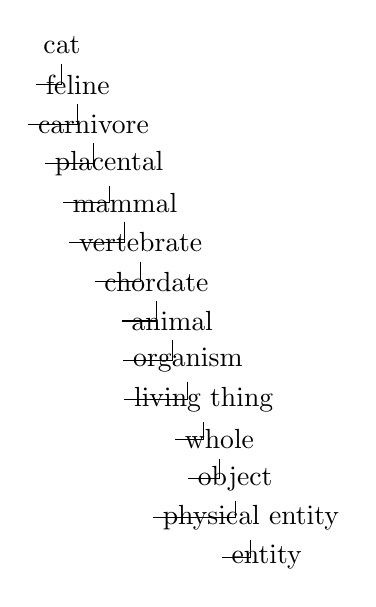
\begin{tikzpicture}[%
  grow via three points={one child at (0.2,-0.5) and %
  two children at (0.5,-0.7) and (0.5,-1.4)},%
  edge from parent path={(\tikzparentnode.south)%
  |- (\tikzchildnode.west)}]
\node {cat}
    child { node {feline}
       child {node {carnivore}
       	child {node {placental}
       	 child {node {mammal}
       	  child {node {vertebrate}
       	   child {node {chordate}
       		child {node {animal}
       		 child {node {organism}
       		  child {node {living thing}
       		   child {node {whole}
       			child {node {object}
       			 child {node {physical entity}
       			  child {node {entity}
          }}}}}}}}}}}}};
\end{tikzpicture}
\caption{Full inherited hypernym tree for 'cat' synset according to WordNet}
\label{fig:hypernym-tree-cat}
\end{figure}

A \textit{meronym} of a synset is a \textbf{part-of} relation. It denotes member constituents of other synsets. For example, the \textit{wheel} synset is a meronym of \textit{car}.


\paragraph{FrameNet}
\label{sec:fn}
FrameNet\cite{baker1998berkeley} is a lexicon with framing semantics to \textit{define and constrain} the building of clauses around individual words. It describes the meaning of a word based on the words that typically participate with it, known as \textit{frame elements} or \textit{FEs}.

Take the Desiring frame for example, which has a list of words, referred to as \textit{lexical units} or \textit{LUs} - that are used in statements that indicate desire, e.g. want, lust, yearn etc. Each of these LUs come with their own \textit{lexical entries} that describe the FEs and \textit{Valence patterns}. These define the types of phrases that can be built around a particular LU.

Take the \textit{yearn} LU. It's FEs and Valence Patterns are shown in Table BLAH:

Table: https://framenet2.icsi.berkeley.edu/fnReports/data/lu/lu6599.xml?mode=lexentry

Valence patterns are grouped by the permutation of FEs, e.g. \textit{Event} and \textit{Experiencer}, or \textit{Experiencer} and \textit{Focal\_participant}. Each group comes with one or more Valence Patterns that indicate the type of phrase (NP means noun phrase, VP means verb phrase etc.), as well as the role in the clause - Ext (Subject), Obj (Object) and Dep (Dependency or Indirect Object).

FrameNet also provides \textit{semantic types} with every FE of a frame. This indicates the required animation of any noun in all Valence patterns of the LU. For example, the \textit{Experiencer} FE is a \textit{Sentient} semantic type, while the \textit{Event} FE has the \textit{State\_of\_affairs} semantic type.

\paragraph{Oxford Collocations Dictionary}
The Oxford Collocations Dictionary\cite{crowther2003oxford} is a source of word combinations. For any given word, it provides the set of words and POS commonly occur in relation to it.

The dictionary entry for \textit{custard} can be seen in Figure BLAH. It gives common adjectives that are used to describe custard and shows that it receives the action of being made, poured and strained, and it takes the actions of thickening and setting. Furthermore, it is closely related to powder and pie.


\paragraph{Associations}
The University of South Florida Free Associated Norms\cite{nelson2004university} provides associations collected directly from human participants. It is used by the Department of Psychology, and is therefore another high quality source of associated words that can be depended on for quality as it was collected in a scientifically sound manner.


\paragraph{NodeBox Perception}
The NodeBox Perception model includes the data used in De Smedt's attempt to model common sense as a network, as discussed in Section \ref{sec:common-sense-bg}. This data was manually entered into the system and continues to be used for research, which means that it is a dependable source of data. 

\paragraph{Google Search Suggestions}
Tony Veale's attempt at modelling metaphors\cite{vealespecifying} introduced a clever use of Google's search suggestions as a method of finding associations between words and ultimately build Metaphor Magnet. While we may not use Metaphor Magnet, we take inspiration from his use of Google's search suggestions.

This is the least dependable source of information that we use because it is dependant on search suggestions rather than structured sentences. Therefore we will use this method with caution.

\paragraph{Noah's ARK Informal Research}
Noah's ARK is an informal research group run by Noah Smith at Carnegie Mellon University\cite{ark} whose research focuses on problems of \textit{ambiguity} and \textit{uncertainty} in natural language processing. They provide online API access to two tools for linguistic structure analysis:
\begin{enumerate}
\item{\textbf{SEMAFOR}\cite{chen2010semafor} for SRL using FrameNet.}
\item{\textbf{TurboParser}\cite{turboparser} for Standford Dependency parsing.}
\end{enumerate}   

SEMAFOR is particularly resource heavy, requiring a minimum of 8 gigabytes of random access memory. However, the request response from the online API is fairly quick - typically 1.24 seconds for simple sentences and 1.61 seconds for complex ones, tested using the specifications in Appendix \ref{sec:specs}.

Noah's ARK request response is in JSON format and includes data from both SEMAFOR and TurboParser. TurboParser returns the Semantic Dependency Parse in CoNLL data format, whose structure can be seen in Table \ref{tab:CoNLL}. 

\begin{table}
\centering
    \begin{tabular}{|l|l|l|}
    \hline
    Field Number & Field Name & Description                                                \\ \hline
    1            & ID         & Token counter, starting at 1 for each new sentence.        \\
    2            & FORM       & Word text form or punctuation symbol                       \\
    3            & LEMMA      & Lemma or stem of FORM                                      \\
    4            & CPOSTAG    & Coarse-grained part-of-speech tag                          \\
    5            & POSTAG     & Fine-grained part-of-speech tag                            \\
    6            & FEATS      & Unordered set of syntactic and/or morphological features   \\
    7            & HEAD       & ID of the parent of the current token ('0' if root)        \\
    8            & DEPREL     & Dependency relation to the HEAD                            \\
    9            & PHEAD      & Projective head of current token                           \\
    10           & PDEPREL    & Dependency relation to the PHEAD                           \\ \hline
    \end{tabular}
\caption{The CoNLL data format output by TurboParser.}
\label{tab:CoNLL}
\end{table}

%----------------------------------------\

\subsection{Natural Language Generation}
\label{sec:bg-nlg}
Natural Language Generation is the term for putting some non-linguistic form of content into understandable text in a human language. Reiter and Dale give the framework\cite{reiter2000building} illustrated in Figure \ref{fig:nlg} for the process of generating natural language.

\begin{figure}[h!]
\centering
\includegraphics[width=30mm]{NLG}
\caption{Reiter and Dale Natural Language Generation process}
\label{fig:nlg}
\end{figure}

A similar model was propsed by Bateman and Zock\cite{mitkov2003oxford}, which includes four stages:
\begin{enumerate}
\item{\textit{Macro Planning:} Overall content of the text is structured.}
\item{\textit{Micro Planning:} Specific words and expressions are decided.}
\item{\textit{Surface Realisation:} Grammatical constructs and order are selected.}
\item{\textit{Physical Presentation:} Final articulated text is presented.}
\end{enumerate}

SimpleNLG\cite{gatt2009simplenlg} is a Java library that provides useful functionality for natural language generation using the ideas of Reiter and Dale. In particular, it enables us to build \textit{phrases} for nouns, verbs, prepositions, adjectives and adverbs that can be enriched with grammatical metadata such as tense, aspect and perspective (for verbs), as well as plurality, gender and animation for nouns.

These phrases can then be put together into \textit{clauses} that define the roles of each phrase in the desired sentence, for example by specifying the subject and object noun phrases. It then \textit{realises} a grammatically correct natural language sentence taking all of the provided information into account.

There are others, such as grammar generation implemented by NLTK (similar to the one used in MCGONNAGAL) or the constraint programming technique used by Toivanen et al. explained in section \ref{sec:con}. However, we find that this process is not granular enough, jumping from the goal to the surface text without enough consideration for the individual words used.

More elaborate tools exist, such as KPML\cite{bateman1997enabling} and FUF\cite{elhadad1989fuf}/SURGE\cite{elhadad1996overview}, that have greater grammatical coverage than SimpleNLG. However, they are either no longer maintained or too complex for our purposes.


% ------------------------------------------------------------------------


%%% Local Variables: 
%%% mode: latex
%%% TeX-master: "../thesis"
%%% End: 

\def\baselinestretch{1}
\chapter{Poem Analysis}
\ifpdf
    \graphicspath{{Theory/TheoryFigs/PNG/}{Theory/TheoryFigs/PDF/}{Theory/TheoryFigs/}}
\else
    \graphicspath{{Theory/TheoryFigs/EPS/}{Theory/TheoryFigs/}}
\fi

\def\baselinestretch{1.66}

The first phase of implementation is to write a suite of algorithms to analyse a single poem in terms of all the features mentioned in section \ref{sec:features}. The aim is to analyse a large collection of poems in such depth to learn the usage patterns of poetic features for that collection of poems. This is in line with the ultimate aim of avoiding hard-coded rules for different types of poems.

The algorithms will cover the detection of the use of:
\begin{itemize}
\setlength{\itemsep}{0pt}
\item{Rhyme and internal rhyme}
\item{Rhythm, including meter and syllable count}
\item{Alliteration, assonance, consonance, onomatopoeia and other sound devices}
\item{Structure, tense, point of view and repetition}
\end{itemize}

Other algorithms will attempt understand the context of the poem to extract:
\begin{itemize}
\setlength{\itemsep}{0pt}
\item{Characters}
\item{Objects}
\item{Locations}
\item{Descriptions}
\item{Relationships}
\item{Actions}
\item{Symbolism including metaphors, similes and personification}
\end{itemize}

The output of this phase is a full analysis of a single poem. In lieu of this, we will walk through the implementations of each of these algorithms using the poems in Figures \ref{fig:cat} and \ref{fig:limerick} as case studies.


\begin{figure}
\centering
\begin{minipage}{0.45\textwidth}
\centering
\textit{
There once was a big brown cat\\
That liked to eat a lot of mice\\
He got all round and fat\\
Because they tasted so nice
}
\caption{A rhyming quatrain often used in teaching poetry}
\label{fig:cat}
\end{minipage}\hfill
\begin{minipage}{0.45\textwidth}
\centering
\textit{
The limerick packs laughs anatomical\\
Into space that is quite economical.\\
    But the good ones I've seen,\\
    So seldom are clean,\\
And the clean ones so seldom are comical.
}
\caption{A limerick about limericks}
\label{fig:limerick}
\end{minipage}
\end{figure}


\section{Obtaining Phonetic Structure}

When poets choose words they take the sound of the words when spoken out loud into account as well as their (literal or symbolic) meaning. As explained in section \ref{sec:words}, we can use CMU Pronounciation Dictionary (CMUPD) to get around the difficulty of determining phonetic structure by spelling. A word in the CMUPD is mapped to a list of different pronunciations for the same word. Each pronunciation is a list of phonemes that make up that particular pronunciation of that word, including indication of emphasis on the syllables as explained in section \ref{sec:words}.

We want to convert the poems into their phoneme lists for use by the detection algorithms. This needs to be done word by word, so we first need to \textit{tokenise} the sentence. Tokenisation involves splitting each sentence into a list of its basic components; words and punctuation. Once we have done that, we can simply iterate through the list and run each word through the CMUPD. Some words have multiple pronunciations, so we consider each possible permutation of pronouncing each line of the poem. Each of the pronunciations of the first line of Figure \ref{fig:cat} is shown in Figure \ref{fig:catpronun}.

\begin{figure}
\centering
[['DH', 'EH1', 'R']] \\
['W', 'AH1', 'N', 'S']\\
[['W', 'AA1', 'Z'], ['W', 'AH1', 'Z'], ['W', 'AH0', 'Z'], ['W', 'AO1', 'Z']]\\
[['AH0'], ['EY1']]\\
[['B', 'IH1', 'G']]\\
[['B', 'R', 'AW1', 'N']]\\
[['K', 'AE1', 'T']]
\caption{The different ways of pronouncing the first line of the cat poem}
\label{fig:catpronun}
\end{figure}

Unfortunately, the CMU Pronunciation Dictionary only has about 133,000 words. This means that occasionally we will fail to translate to the phonetic structure, particularly in Shakespearean poems. We get around this by temporarily converting the word into its closest match that exists in the dictionary and returning the phonetic structure in its place.

Python difflib provides a function to find the closest matches of a word to a list of words, based on the Ratcliff/Obershelp pattern recognition algorithm. The complexity of this algorithm is quadratic in the average case and cubic in the worst case. However, difflib's implementation avoids this using a 'junk' heuristic and hashing so the worst case becomes quadratic and the best case linear. The behaviour is based on  how many sequences have in common. Since we are only dealing with single words at a time, we have a higher chance of the best case. On average it takes X MILLISECONDS to look up a 4-letter word and Y MILLISECONDS to look up an 8-letter word, which is easily fast enough given that speed is not a priority for this phase since it is a pre-processing phase, not a time-sensitive one.

We could use a variety of other techniques to get around this problem other than string matching:
\begin{itemize}
\item{Break many syllable words into likely part-words, e.g. 'thrift' and 'less' instead of 'thriftless'}
\item{Try all combinations of stress and syllables}
\item{Train a finite-state transducer model as in \cite{dobrivsek2010towards}}
\end{itemize}

The first option only works in a limited number of situations that are reasonably handled by the string matching solution. For example, 'thriftless' would become 'shiftless', which has an identical phonetic structure. The second option can result in poor performance and more false negatives or false positives than would be worth the added processing.

The final option is the most viable and would be used if the generation phase depended on perfect readings of the poems, as the stochastic n-gram methodology of RKCP would. However, as we only use this as an approximation for abstraction in later phases, we can afford to use a more naive implementation.


\section{Rhyme}

We want to detect end-line and internal rhyme, as described in section \ref{sec:rhyme}. Along with detecting it, we want to be able to build a normalised rhyme scheme representation for easy analysis in the abstraction phase. 

First we collect the phoneme set of the words that we wish to analyse for rhyme. For end-line, we collect the last word of each line of the poem. For internal rhyme, we collect the all the words in a particular stanza.

Once we have our list, we can run it through Algorithm BLAH.

1 for each word in the list:
2 	for each pronuciation of the word:
3		for each phoneme in the pronunciation:
4			if this phoneme is stressed:
5				get all the rhyme phoneme pattern from this phoneme onwards in this pronunciation
6				if we have seen this pattern before: 
7					assign it corresponding rhyme token
8				else:
9					map this pattern to a new rhyme token
10				
11				append this token to a set of possible tokens for this word				
12	append the set possible tokens for this word to the unzipped rhyme scheme
13 build all possible permutations of rhyme scheme from they unzipped rhyme scheme
14 normalise the rhyme schemes
	
There are a few tricks to this algorithm, namely obtaining the rhyme phoneme pattern on line 5 and the process of building and normalising the rhyme scheme in lines 11 to 14.

\subsection{Obtaining the Rhyme Phoneme Pattern}

Two words rhyme when:
\begin{itemize}
\item{the last phoneme of each word match}
\item{the vowel sounds after and including the first stressed syllable match \textbf{in order}}
\end{itemize}

The algorithm finds the first stressed syllable in line 4. At that point we only need to iterate through the rest of the pronunciation and find the vowel sounds and the last phoneme check that the last phonemes. Putting them together in order gives the unique rhyme phoneme pattern. 

For example strategy and tragedy, kite and height - colourful diagrams!			

\subsection{Building and Normalising the Rhyme Scheme}

Each unique rhyme phoneme pattern is represented by a single capital letter starting with 'A'. This is matches with the standard convention for rhyme schemes used in theory. 

The complication comes in the various ways of pronouncing a single word. Therefore, we create a list for every possible rhyme pattern for a each word. The list of these lists is what the algorithm refers to as the 'unzipped' rhyme scheme on line 12 and 13. Figure BLAH shows the unzipped rhyme scheme for the limerick in Figure BLAH. Not that the word 'anatomical' has two pronunciations that affect the rhyme pattern, according to the CMUPD.

FIGURE OF THE UNZIPPED RHYME SCHEME

We then build every possible permutation of this list, which then gives us a list of the possible rhyme schemes for these given words. We leave this list as it is and do not make a claim for any rhyme scheme to be more likely than any other at this stage.

\section{Rhythm}

We attempt to recognise all three types of rhythm described in \ref{sec:rhythm}. 

\subsection{Detecting Syllabic Rhythm}

The number of syllables in a word is equal to the number of vowel phonemes it has. We know that all vowel phonemes have a stress marker appended to it so we can just count the number of stress markers in the word.

However, Syllabic Rhythm is done on a line-by-line basis. Therefore we tokenise each line and aggregate the vowel phonemes across all words in the line to get the number of syllables for that line.

If we take one permutation of the line in Figure \ref{fig:catpronun}, we can see that each word has one vowel phoneme, so each word in that sentence is monosyllabic. Therefore the number of syllables in the line is 7.

The full syllabic rhythm for the poems in Figure \ref{fig:cat} and \ref{fig:limerick} are 7-8-6-7 and 11-6-5-11-11 respectively. We represent these as a list of integers. We create a separate list for each stanza.

\subsection{Detecting Quantitative and Accentual Rhythm}

While theory counts rhythm in terms of metre and feet, as described in \ref{sec:rhythm}, some poems might have rhythm without following one of these pre-defined popular styles. Instead of searching for them, we will extract the pattern of stressed and unstressed syllables for each line without making a claim on how it matches to theory yet.

We choose to do this mainly because there could be multiple possibilities for the stress pattern of a line due to variations in emphasis for particular words, e.g. '\textbf{ob}ject' and 'ob\textbf{ject}'. The variability of possible stress patterns is compounded by some limitations of the CMUPD:
\begin{itemize}
\item{Some words are restricted to a single stress pattern even though it does not lose or change the meaning of the word if it was emphasised differently. For example, '\textbf{quan}tity', 'quan\textbf{ti}ty' and 'quanti\textbf{ty}' are all valid, but the CMUPD only recognises the first because the other two are unusual in normal speech (but not for poetry).}
\item{Similarly, the CMUPD fixes monosyllabic words to one of stressed or unstressed as in Figure \ref{fig:catpronun}. However, they can be either so we need to allow for both possibilities.}
\item{Stresses on some words have changed over time. For example \textbf{prov}ed was pronounced prov\textbf{ed} in Shakespeare's era}
\item{Though not necessarily a limitation, we do not give importance to light or secondary stress in a word (the '2' stress marker). We therefore assume it could be either '1' or '0'.}
\item{Poetic license often allows words to be pronounced with an entire extra syllable. For example \textit{de-served} could be pronounced as \textit{de-ser-ved}.}
\end{itemize}

We account for these by increasing the number of possible readings. However, this will lead to a lot of possibilities. For example the line in Figure \ref{fig:catpronun} will give us any combination of '1's and '0's since they are all monosyllabic and by the second point above we want to allow for either. 

We narrow this down initially by taking away any occurrences of the same stress three or more times in a row in the same line, because no one will ever read a poem in this way.  Like with rhyme, we do not make a claim for any stress pattern to be more likely than any other at this stage.


\section{Sound Devices}

We aim to detect each of the sound devices described in \ref{sec:sound}.

\subsection{Detecting Consecutive Sounds}

RETHINK THIS IMPLEMENTATION

For assonance, consonance and alliteration, we only care about whether or not they are being used, not necessarily which sounds are repeated or where in the poem it occurs.

\subsection{Onomatopoeia}

Some onomatopoeia are recognised in traditional dictionaries, while some are not. There are also many variations of the same sound, e.g. 'Aah' versus 'Aaah'. New onomatopoeia can be created at any point depending on the sound the writer wants to portray. This range of variation and lack of consistency makes it difficult to detect all occurrences of onomatopoeia.

However, we can use the WrittenSound.com dictionary of onomatopoeia to recognise the most common ones. We can check each word in the poem for existence in the dictionary or for a very similar words to those in the dictionary. To do this we can use the Levenshtein distance, a measure of the number of changes required to turn one string into another. If the Levenshtien distance between a word and an entry in the dictionary is less than or equal to 1, not including extensions to the head or tail of the onomatopoeia, then we consider it to be onomatopoeic.

Furthermore, WrittenSound has mappings between the onomatopoeia and the type of sound they represent. For example, \textit{'ding'} represents a 'hard hit', probably of a 'metal' object. This can be useful somehow.


\section{Form and Structure}



\subsection{Stanzas, Lines and Sentences}

\subsection{Point of View}

\subsection{Tense and Aspect}



\section{Context and Pragmatics}
Here we describe the approach to the difficult challenge of determining the context of the poem in terms of its characters and their relations, descriptions etc. as described in section \ref{sec:pragpers}. The aim is to build a representation of the characters much like a human reader would in their mind. This will then be compared in the abstraction section to find a correlation between these structures and types of poetry.

\subsection{ConceptNet Relations}
ConceptNet is a semantic network of '\textit{general knowledge}'. Each node in the network is a natural language word or phrase called a \textit{concept}. Edges in the network represent a relationship between two concepts. These relationships come in various types, for example:

**Big list of the relations with the ones that we are concerned with at the top.**

We can use these relationships to build a cohesive story about particular characters during the generation phase. However, in keeping with the theme of this paper we cannot simply hard-code or randomise this process. Therefore, we need to be able to analyse these relationships in existing poems during the abstraction phase to find correlations. For example, we may find that descriptive poems have a high number of \textit{HasProperty} relations and very few characters.  

To do this, we need to be able to extract relationships between concepts in a particular poem in lieu of ConceptNet relations. For example:

**Give the cat example**

\subsection{Semantic Labelling using Noah's ARK}

It would be very difficult to determine these relationships from a syntactical parse alone. This is due to the complex nature of the English language, in particular verb usage. For example, the phrase \textit{tasted so nice} is a description rather than an action because the word \textit{tasted} in this case is being used as a linking verb, where it is usually an action verb.

These complexities are further compounded by the fact that we cannot rely on correct grammar in poems. We therefore need a \textit{semantic} parse. Noah's ARK is an informal research group run by Noah Smith at Carnegie Mellon University. They provide online API access to two tools for linguistic structure analysis, \textit{SEMAFOR} and \textit{TurboParser}. Both of these tools in conjunction are satisfactory for our aim to extract ConceptNet relations from natural language.

\subsubsection{FrameNet Semantic Role Labelling using SEMAFOR}
\label{sec:sema}

Semantic Role Labelling (SRL) is best described with an example. Take the sentence \textit{"The shopkeeper told the hoodlum to go away"}, we wish to recognise the verb \textit{'to tell'} as the target, \textit{'the shopkeeper'} as the speaker, \textit{'go away'} as the message and \textit{'the hoodlum'} as the addressee. This can be seen clearly in Figure BLAH. 

This is independent of the syntactic structure of the sentence and does require grammatical correctness. The SRL for the \textit{'Yoda-speak'} equivalent will remain the same, as shown in Figure BLAH.

These labels are retrieved through the SEMAFOR tool, which was trained on FrameNet data to determine the frame-semantic structure of the text. FrameNet is a lexical database of \textit{semantic frames}, which describe the meaning of a word based on the words that typically participate with it, known as frame elements. It is based on the Frame Semantics Theory, introduced by Charles J.Fillmore et al.

We can use these to derive the ConceptNet relations by looking for the occurrence of frames, and elements thereof, that correspond to the ConceptNet relation. These manually chosen lists can be found in THE APPENDIX. However, each list may not be exhaustive for its corresponding ConceptNet relation and there are some relations that will not be picked up by this method.


\subsubsection{Semantic Dependency Relations using TurboParser}
\label{sec:turbo}

The Stanford Dependencies is another representation based around the relationships between words. All dependency relations are strictly binary and come in various types depending on the participants (called the \textit{governor} and the \textit{dependent}).

The semantic dependency tree for the previous shopkeeper example can be seen in Figure BLAH.

This representation fills the gaps left by the frame-semantic parse using the following heuristics:

PSEUDO-CODE HEURISTICS HERE

Together, these tools provide a fairly complete coverage of the ConceptNet relations.


\subsection{Extracting and Binding Relations to Characters}

At this point, the derived ConceptNet relations are only a set of abstracted FrameNet frames and matched dependencies. This alone does not give us much more information than if we were to use the frame-semantic parse on its own. The true usefulness of this approach only arises if the relations can be bound to characters of the poem. For the shopkeeper example, we would recognise \textit{the shopkeeper} and \textit{the hoodlum} as objects with SendMessage and ReceiveMessage relations bound to each of them respectively with respect to the \textit{go away} message.

We can represent the desired output as a set of 'hubs', with each character at the centre of the hub as in Figure BLAH. This will also improve our knowledge for the generation phase in that we will know the \textit{number} of characters typical for a poem type, the \textit{number and type} of relations associated with \textit{each} character, as well as allow us to find commonalities in the types of characters themselves.

To reach the desired representation, we execute Algorithm BLAH:

1 for each sentence in the poem:
2   get the dependency relations and frame semantic parse
3	collapse loose leaves of the dependency relations
4	find and create possible characters
5	find candidate ConceptNet relations from the frame-semantic parse
6	for each character:
7		get all associated dependency relations
8		for each associated dependency relation:
9			if the dependent is involved in a candidate relation from the frame-semantic parse:
10				bind the relation to the current character and continue
11			else:
12				use the heuristics for dependency relations to find possible ConceptNet relations
13				bind any that are found to the current character and continue
				
Here we describe each step in detail.

\subsubsection{Obtaining the Semantic Dependency Relations and Frame-Semantic Parse from Noah's ARK}

Noah's ARK provides parse data from both SEMAFOR and TurboParser in a JSON format that can be accessed by sending a request to their demo API. However, there is a cap of 20 seconds processing time for any request so we only send one sentence at a time to be safe. Some basic experimentation has shown that this does not hinder accuracy.

SEMAFOR returns the Frame-Semantic parse in JSON format, an example of which can be seen in Figure BLAH. We leave it in this format because we only need to access this data once when finding the candidate relations on line 5 of Algorithm BLAH.

TurboParser returns the Semantic Dependency Parse in CoNLL data format, whose structure can be seen in Table BLAH. An example of the output can be seen in Figure BLAH.

We parse this into a simple dependencies dictionary format shown in Table BLAH for easy access and processing downstream. 

TurboParser and SEMAFOR are resource heavy (SEMAFOR requires minimum 8GB RAM), so it makes sense to run it on a server. Since the output from Noah's ARK is exactly what we want and the request is fairly quick (typically BLAH milliseconds for simple sentences, BLAH milliseconds for complex ones) and speed is not a priority for this project, there is no need to run our own copy on our own server.

\subsubsection{Collapsing Loose Leaves of the Semantic Dependency Relations}
\label{sec:collapse}

In a lot of cases, the character or relation that we look for is a phrase, not just a word. For example in Figure BLAH the character should be \textit{a lot of mice} rather than just \textit{mice}. In fact if we skipped this step, we would get two characters; \textit{a lot} and \textit{mice}, which is obviously wrong.

Another example is the phrase \textit{tasted so nice}. If we did not collapse the tree, we would have that \textit{they} took the action of \textit{tasted} and can be described as \textit{nice}, both of which are wrong again.

The non-demo version of TurboParser provides different styles of dependency representation. This includes collapsed dependencies but not exactly in the way we want it done. First, we manually select the dependencies that we want to collapse:

LIST OF DEPENDENCIES TO COLLAPSE

By default, the parent of the dependency keeps all its attributes unchanged except for merging its form with that of the leaf, e.g. \textit{of} and \textit{mice} becomes \textit{of mice}. However, there are some cases where we wish to retain the part-of-speech (POS) tag of the leaf and overwrite the parent's part of speech tag. For example, \textit{of mice} should retain the 'NNS' POS tag of \textit{mice} rather than keep the 'PRP' POS tag of \textit{of}. The full list of these conditions are:

LIST OF CONDITIONS TO RETAIN POSTAG FROM LEAF

Then we follow Algorithm 2:
1 Get a list of all the leaves in the graph.
2 For each leaf in the reverse of this list:
3	If the dependency relation of this leaf (i.e. from its parent) is collapsable:
4		Get the parent
5		Merge the form of the parent and the leaf
6		If necessary, the parent retains the part-of-speech tag of the leaf
7		The leaf is destroyed and the parent becomes the leaf.
8		Loop back to line 3.

Figure BLAH shows a dry run of this algorithm on the sentence \textit{"There once was a big brown cat who liked to eat a lot of mice."}

\subsubsection{Finding and Creating Characters}
\label{sec:characters} 

A naive method for finding characters would be to look for nouns and pronouns to recognise characters in a poem. This would actually be sufficient, but we can do better. Notice in the poem in Figure BLAH, the cat character is represented by the words \textit{'a cat'} and \textit{'he'}. Similarly, \textit{'a lot of mice'} and \textit{'they'} represent the same character.

In Computational Linguistics, this problem is called \textbf{Anaphora Resolution}. It is an ongoing research area and I will present a new potential solution in section \ref{sec:ar}.

Part of the solution is gathering some basic semantic information about the character. We would like to determine whether the character:

\begin{enumerate}
\item{is plural or singular.}
\item{is male, female, neutral or unknown.}
\item{the character is an animate/living object, an inanimate physical object or a non-object.}
\end{enumerate}

The first point is easiest:
\begin{itemize}
\item{If it is a noun and the part-of-speech tag ends in an 'S', it is plural.}
\item{If it is a pronoun, check for membership in the manually built list of plural pronouns (e.g. 'they', 'them').}
\end{itemize}

The pronoun case for the second point is similar; we check for membership in the manually built list of male pronouns (e.g. 'he', 'him') and the separate list of female pronouns (e.g. 'she', 'her'). 

The noun case is trickier. First we need to find the \textit{synset} of the noun. Synsets are sets of cognitive synonyms, e.g. \textit{car} and \textit{automobile} are in the same synset, but not \textit{cable car}. Once we have this, we can use the hypernym relationships between synsets.

A hypernym of a synset is a \textbf{type-of} relation. For example, the synset \textit{mammal} is a hypernym of \textit{cat} because cat is a type of mammal. Similarly, \textit{animal} is also a hypernym of cat, as well as being a hypernym of mammal. The full hypernym tree for \textit{cat} can be seen in Figure BLAH. 

The \textit{direct hypernym} of a synset is the synset directly above it in the hypernym tree; \textit{feline} in the case of the cat. The \textit{inherited hypernym} of a word refers to any word that appears in its hypernym tree. WordNet, a lexical database of the cognitive relations between words provides all of these resources.

Now, finally, we can check for whether a noun is male or female by looking for the existence of particular synsets that imply a gender. For example, the \textit{'female'} synset would be an inherited hypernym of the synset \textit{'cow'}. Therefore we know that cows are female. Similarly, \textit{'maharaja'} has the hypernym \textit{'prince'}, which we know to be male.

We can extend this practice to the final point of determining the animation of the character by checking if the \textit{'living thing'} and \textit{'physical object'} synset is an inherited hypernym of the synset of the noun concerned.


\subsubsection{Extracting Candidate ConceptNet Relations from the Frame-Semantic Parse}
\label{sec:candidate}

As mentioned in section \ref{sec:sema}, we have a manually built map between FrameNet frames and ConceptNet relations. Given this, we can carry out Algorithm BLAH.

1 for each frame found in the frame-semantic parse:
2	look up the target of the frame in the map
3	if it can help build a ConceptNet relation:	
4		retrieve the frame elements
5		replace the frame elements with the corresponding text from the poem
6			if we cannot find all the elements we are looking for, we leave it blank
7		add mapping from the text of the frame target to the newly built relation
	
Let us take the shopkeeper example from earlier. If it exists, we then look for the specific frame elements that will allow us to build the ConceptNet relation.

GO THROUGH THE SHOPKEEPER EXAMPLE

\subsubsection{Obtaining the Associated Dependency Relations for a Particular Character}

This step breaks up the semantic dependency tree and flatten it into the character-centric hubs as shown in Figure BLAH.

First, we want to identify the character in the dependency tree. All of the relations going out from it are naturally related dependencies of the character, so they get added to the list, see Figure BLAH.

The single relation coming into this character is also a related dependency, so we added that to the hub and reverse the direction of the branch, see Figure BLAH.

Now we have a tree with the character as the root. The next step is to flatten it so that everything is related to the character. We do this by recursively converting all the grandchildren of the character root node to a direct child node until there are no more grandchildren. This process is illustrated in Figure BLAH.

We repeat this process for each character starting from the leftmost character in the sentence. However, we quickly notice that there will be duplication; the same dependency will be associated to more than one character. To avoid this, we can prune these hubs by working backwards through the list of characters (i.e. starting from the rightmost in the sentence) and removing duplications in earlier nodes, as shown in Figure BLAH. 

This works because the head of the last character will be lower down in the tree than the head of any other character. This has the effect of removing the duplicated dependencies such that the last one standing is only associated to the one it was closest to in the original tree.


\subsubsection{Binding ConceptNet Relations to Characters}
	
Now that we have our hub data structure for all characters, we now need to look at each branch and of each hub and decide if it can be converted into a ConceptNet relation.

First, we check if the text of the child maps to one of the candidate relations we extracted from the frame-semantic parse in section \ref{sec:candidate}. If it does, then we accept that and move on to the next child without checking the dependency relation since it is likely to be the more accurate. Sometimes the dependant of the relation will be blank because we could not find the right frame element as explained earlier. In this case, we just assume that this is a relation to the next character in the characters list. This is a fair assumption given the limited number of characters per sentence, the general forward reference structure of sentences and the fact that most of the relations we look to build are between characters.

If there is no candidate relation for this child, we then look at the type of the dependency between it and the character. We use the heuristics described in section \ref{sec:turbo} to convert it into a ConceptNet relation.

If we cannot find a relation through either of the above methods then it is likely there isn't one, so we remove it from the hub.

In all of those steps, we need to look out for negative adverbs such as 'not', 'seldom', 'rarely' etc. which we use to negate the ConceptNet relation found. We also need to look out for antonyms in the target word in the frame-semantic parse. For example, the \textit{Experiencer-focus} frame helps us find \textit{Desires} and \textit{NotDesires} ConceptNet relations depending on whether the target word is synonymous with 'love' or with 'hate', for example.

We can see this final step being applied to our ongoing example in Figure BLAH.


\subsection{Anaphora Resolution}
\label{sec:ar}
We can now clearly see the anaphora problem as described in section \ref{sec:characters}. We must match up the \textit{'a cat'} character and \textit{'he'} character, and the \textit{'they'} character with the \textit{'a lot of mice'} character. 

In this particular example, we can simply match the plurals and singulars together. However, we may not always be so lucky. We may also run into a situation where the cat could be referred to as \textit{'the feline'} instead of \textit{'he'}.

Section \ref{sec:arback} gives an overview of the state of the art solutions. Our solution is also pretty darn simple at the moment, so I am going to wait to see if I can do some of the more complicated things and then write this section up.


\subsection{Peeks at Future Development of Pragmatic Language Analysis}

If I get time...


\section{Symbolism and Imagery}

This particular poetic technique can be very subtle and difficult to detect. Of the ones listed in section \ref{sec:symbol}, we are able to recognise the use of two; similes and personification.

\subsection{Personification}

We used the animation state of characters for anaphora resolution. We can take this idea further to detect the use of personification in poetry.

The following relations are symptomatic of a sentient being:

LIST OF ANIMATE RELATIONS

Therefore, if a character that is marked as an inanimate physical object has any of these relations, it is likely that the author of the poem was using personification to give the object human-like behaviour.

We can also take advantage of the \textit{Semantic Type} attribute of FrameNet elements. FrameNet marks frame elements with a semantic precondition if they are to be of a certain type, for example only \textit{'Sentient'} semantic types can be the \textit{'Abuser'} and the \textit{Victim} in the \textit{'Abusing'} frame. By looking up these semantic types in FrameNet as we are building the ConceptNet relations, we are able to flag characters as evidence for personification.

\subsection{Simile}

Similes are relatively easy to detect because they often use the phrases 'like a' or 'as a' and 'than'. They also follow certain syntactical patterns in that it is usually a noun followed by a verb or adjective, then one of the aforementioned phrases, followed by a noun or an adjective.

A particular symptom of simile use is that the aforementioned phrases will be involved in a prepositional noun phrase, or 'PNP Chunks' to use the parser terminology.

We could take this further by using ConceptNet btw. As fast as a cheetah + cheetah HasProperty fast -> simile.

\subsection{Metaphor}

We need to do something here. Can't just leave it...

\section{Optimisation}

%%% ----------------------------------------------------------------------

% ------------------------------------------------------------------------

%%% Local Variables: 
%%% mode: latex
%%% TeX-master: "../thesis"
%%% End: 

\chapter{Analysis Interpretation}
\ifpdf
    \graphicspath{{Implementation/ImplementationFigs/PNG/}{Implementation/ImplementationFigs/PDF/}{Implementation/ImplementationFigs/}}
\else
    \graphicspath{{Implementation/ImplementationFigs/EPS/}{Implementation/ImplementationFigs/}}
\fi

The second phase of implementation involves interpreting the results of the analysis phase. The goal is that these interpretations can be used to template the structure and outline the content for certain collections of poems, ultimately guiding the generation of novel and authentic poetry in the final phase.

\section{Approach}
\label{sec:balance-priorities}

In deciding how to approach this phase, we need to make predictions about the usage of the final interpretation and assumptions about the quality, or lack thereof, of the corpus and analysis.


\subsection{The Corpus}

The corpus is a large collection of poems. We may assume that each poem is already marked with the \textit{type} of the collection - limerick, haiku, riddle etc. - much like data in a supervised machine learning problem. However, the poems should otherwise be \textit{unseen} before analysis; we know nothing else about them. 

Poems are most easily obtained from anthologies. This works very well with our assumptions as the data is already labelled with the type of poem, but we know nothing else about the content.

Another way to gather poems is by looking for those freely available on the Internet. However, the corpus obtained from an Internet search will likely be of lower quality than directly from a published anthology. For example, we may get the limerick in Figure \ref{fig:awkward-limerick}, which is clearly very awkward. We can immediately see that it does not follow the typical \textit{'AABBA'} rhyme scheme, and even more so that it doesn't have a fifth line!

\begin{figure}[h!]
\centering
\textit{
A limerick fan from Australia\\
regarded his work as a failure:\\
his verses were fine\\
until the fourth line\\
?
}
\caption{A very awkward limerick for analysis}
\label{fig:awkward-limerick}
\end{figure}
Nevertheless, our blindness to the content of the corpus means the system must be robust to such outliers. Therefore, we \textit{will} get anomalous results and need to be able to cope with them.

\subsection{Subcategories of Collections}

The first two stages aim to be an exhaustive analysis of any type of poem. The first stage achieves this by detecting as many features in a single poem as possible. The second stage does this not only by finding highlights among features of homogeneous poems, but correlations between them as well.

For example, limericks that start with \textit{'There was a...'} may have a very distinctive rhythm pattern for the first line that is otherwise not strictly followed. Therefore, when generating new poetry in the next phase that starts with \textit{'There was a...'}, we want to make sure we abide by this correlation.

There will be many correlations with more than two variables that may be more difficult to spot, but the complexity of finding all of them is exponential. We need to find a balance between the usefulness of this data and the complexity in obtaining it.

\subsection{Novel and Creative Generation}

There is another catch to the correlation problem - red herrings. Some features can be taken as law; 5 lines in a limerick, 5-7-5 syllable pattern in Haiku, iambic pentameter in Shakespearean Sonnets. However, some may be coincidences or the result of a very biased corpus.

Furthermore, we want to be able to generate poems that are \textit{novel} and \textit{creative}. So while we need to be guided by prior art on structure and content to create authentic pieces of literary art, we need to balance that with freedom of creativity. 


\section{A Stochastic Approach}
\label{sec:approach}

The most suitable implementation that meets the priorities listed above is:
\begin{itemize}
\item{Analyse each poem individually as planned.}
\item{Store collections of poems by type (limerick, haiku etc.). This avoids extra filtering and repeated memory persistence downstream.}
\item{Put the analysis results of each poem in a particular collection together, keeping each feature independent. For example, we put all of the rhyme schemes for all limericks in one big list, saving it separately from the list of stanza lengths. I will refer to this step as \textit{'aggregation'} from now on.}
\item{For each feature, create a probability distribution of the results that represents the likelihood of any particular value occurring for each feature. If 95 out of 100 limericks have an \textit{AABBA} rhyme scheme, then we consider the probability of an \textit{AABBA} rhyme scheme in a limerick to be 95\%.}
\end{itemize}

The aggregation step is bespoke to each feature. For example, we aggregate the tenses for each line of each poem differently to the way we would aggregate the overall tense for each poem. This enables us to handle outliers on a case-by-case basis since they are defined differently for every feature.

We can also decide how to \textit{interpret} the data on a case-by-case basis, helping us handle the varying error bands for each feature. For example, detecting the rhyme scheme is more error-prone than detecting the number of syllables so we may round a 95\% result for rhyme scheme up to 100\%, but take it literally for syllable pattern.

This implementation also gives an effective way of finding correlations. We take a value for one of the features as a \textit{given}, filter the store of analysed poems by this value and aggregate. We can take any number of given values and of any permutation since each feature is aggregated and interpreted in isolation.

As a bonus, this implementation quite efficient both in terms of time and space (see Section \ref{sec:interpret-perf}). By storing the original poem analysis results, we can apply given values and find correlations \textit{lazily}, i.e. only when needed.


\section{Algorithms}

All features can be aggregated using some variant of one of four algorithms, with slight feature-specific amendments so to have the flexibility and precision mentioned in the previous sections.

\subsection{List Comprehension}
\label{sec:listcomp}

The simplest of the four algorithms utilises Python's built in functional programming feature; list comprehensions. In a single line of code we put all of the results for a particular feature from all poems in the collection into one big list. Algorithm BLAH shows the code for aggregating the number of stanzas.

\textit{
1. num\_stanzas = [poem.n\_stanzas for poem in poems]\\
2. return Count(num\_stanzas)
}

The second line gets the frequency distribution of this list, which can easily be turned into a probability distribution as required.


\subsection{Line by Line}

Sometimes we can gain more insight by interpreting patterns in a feature for \textbf{each line} rather than the poem altogether. In these cases, the analysis result is usually saved in the form of a tuple, one entry for each line.

Take stress patterns for example. The analysis of a single poem will store the result as \texttt{(x$_1$, x$_2$, ..., x$_n$)} where \texttt{x$_i$} is the stress pattern for line \texttt{i} up to the total number of lines in that poem, \texttt{n}.

Suppose we have three poems in the corpus altogether. Then we have three tuples to aggregate: \texttt{(x$_1$, x$_2$, ..., x$_n$)}, \texttt{(y$_1$, y$_2$, ..., y$_n$)} and \texttt{(z$_1$, z$_2$, ..., z$_n$)}. 

If we are looking generalise the results on a line by line basis, we want to \textbf{transpose} the data to group each line together and put them in a list with the format \texttt{[(x$_1$, y$_1$, z$_1$), (x$_2$, y$_2$, z$_2$), ... ,(x$_n$, y$_n$, z$_n$)]}.

Once this is done, we can apply the list comprehension algorithm described in Section \ref{sec:listcomp} to each tuple in the list. Algorithm BLAH outlines this full process with the stress pattern example.

\textit{
1. stress\_patterns = [poem.stress\_patterns for poem in poems]\\
2. stress\_patterns\_all\_lines = transpose(stress\_patterns)\\
3. return [Count(stress\_pattern\_single\_line) for stress\_pattern\_single\_line in stress\_patterns\_all\_lines]\\
}
\subsection{Pick the Most Popular}

The analysis of a single poem often has some ambiguities. For example, the rhyme scheme for a collection can never be decided by looking at just one poem because words can be pronounced in more than one way. The limerick in Figure \ref{fig:ambiguous-rhyme} could either be \textit{AABBA} or \textit{AABBC} because \textit{invited} can be pronounced as \textit{[IH N V AY T \textbf{AH} D]} or \textit{[IH0 N V AY T \textbf{IH}, D]} according to the CMU pronunciation dictionary.

\begin{figure}[h!]
\centering
\textit{
There was a young man so benighted\\
He never knew when he was slighted;\\
He would go to a party\\
And eat just as hearty,\\
As if he'd been really invited.\\
}
\caption{A limerick with more than one possible rhyme scheme}
\label{fig:ambiguous-rhyme}
\end{figure}

The analysis phase does not make a claim on which rhyme scheme is accepted and instead stores all possibilities in a list \texttt{[x$_1$, x$_2$, ..., x$_n$]}, where \texttt{x$_i$} is the $i$\textsuperscript{th} rhyme scheme possibility up to \texttt{n} possibilities for the particular poem being analysed.

Let's assume again that we only have three poems in the corpus. Once they are all analysed, we get three lists \texttt{[x$_1$, x$_2$, ..., x$_n$]}, \texttt{[y$_1$, y$_2$, ..., y$_n$]} and \texttt{[z$_1$, z$_2$, ..., z$_n$]} of possible rhyme schemes for each poem.

We illustrate what we want to happen by taking four cases:
\begin{itemize}
\item{All possibilities across all poems are unique. Therefore, all are equally probable and that gives us our probability distribution.}
\item{There is \textit{one} set of indices $(p, q, r)$ such that \texttt{x$_p$} == \texttt{y$_q$} == \texttt{z$_r$}. Then we take that to be the rhyme scheme and no other possibility is considered.}
\item{There is $m$\textit{\textgreater 1} sets of indices $(p_1, q_1, r_1), (p_2, q_2, r_2), ..., (p_m, q_m, r_m)$ such that for all $i$ up to $m$, \texttt{x$_{p_i}$} == \texttt{y$_{q_i}$} == \texttt{z$_{r_i}$}. Then all \textbf{sets} are candidate rhyme schemes where each rhyme scheme has a probability of $1/m$.}
\item{There is a $p$ and a $q$ such that \texttt{x$_p$} == \texttt{y$_q$}, but no $r$ such that \texttt{y$_q$} == \texttt{z$_r$}. In this case, the rhyme scheme \texttt{x$_p$} has a probability of two thirds, while every rhyme scheme \texttt{z$_i$} has the probability of one third each.}
\end{itemize}

An iterative implementation makes this process simple. We first find the most popular rhyme scheme among all poems in a set and save its frequency. We then remove all poems that contain the most popular rhyme scheme from the set and repeat on the remaining poems until there are no more poems in the set. 

Algorithm BLAH shows the pseudo-code for this implementation.

\textit{
 1. rhyme\_scheme\_counts = \{\}\\
 2. possible\_rhyme\_scheme\_lists = [poem.rhyme\_schemes for poem in poems]\\
 3. all\_possible\_rhyme\_schemes = flatten(possible\_rhyme\_schemes)\\
 4. most\_popular\_rhyme\_schemes = most\_common(all\_possible\_rhyme\_schemes)\\
 5. for each rhyme\_scheme in most\_popular\_rhyme\_schemes\\
 6. 		rhyme\_scheme\_counts[most\_popular\_rhyme\_scheme)] = all\_possible\_rhyme\_schemes.count(rhyme\_scheme)\\
 7. for each possible\_rhyme\_scheme\_list in possible\_rhyme\_scheme\_lists\\
 8.		if possible\_rhyme\_scheme\_list contains any of  most\_popular\_rhyme\_schemes\\
 9.			remove possible\_rhyme\_scheme\_list from possible\_rhyme\_scheme\_lists\\
10. if possible\_rhyme\_scheme\_lists is not empty, go to 3.\\
11. return rhyme\_scheme\_counts\\
}

\subsection{Filter Below Threshold}

This algorithm deals mostly with content-based features such as n-grams, persona relations and types of persona. These features are varied, unpredictable, error-prone and highly sensitive to bias in the corpus. However, they can still provide very interesting and useful data to guide generation and create authentic poems. For example, starting a limerick with \textit{'There was a...'} and talking about nature in Haikus.

In this case, we perform the most suitable of the three aforementioned algorithms to collect all possible results. We then apply a filter so that only results that occur with \textit{significant frequency} can be taken into account.

Unfortunately, there is no way to tell what frequency can really be counted as significant. It will vary greatly between types and subcategories of poems and is prone to many red-herrings. Trial and error has given the optimal threshold of 9\% of the corpus, but this will need further research to refine.

\section{Testing and Validation by Inspection}

We test and validate this phase by looking at two factors:
\begin{enumerate}
\item{Accuracy of the assumptions and predictions made at the start of this chapter.}
\item{Comparison of results with known poetry theory.}
\end{enumerate}

While some automated tests can be written to make sure that the algorithms above are implemented correctly, there is no desired output against which to compare. We cannot check for exact matches with poetry theory because this is an \textit{investigation} where known theory is the hypothesis. Writing tests that fail if the hypothesis is not correct is an investigative fallacy.

Therefore, the best way to test and validate the results of this stage is by inspection. Python provides a convenient interface for graphing large sets of data, which also make it easy to inspect by eye. 

The corpus used to test the system comprises of 450 limericks scrounged from the Internet. As mentioned earlier, poems gathered from the Internet are likely to have more outliers and anomalies, which makes for a more rigorous examination of the quality of our analysis and interpretation. 

A noteworthy subset of the results are shown in Figures \ref{fig:rhyme-scheme-chart} through \ref{fig:overall-tense-chart}. The y-axis is given in raw values instead of probabilities for this testing stage.
\newcommand{\exedout}{%
  \rule{0.8\textwidth}{0.5\textwidth}%
}

\begin{figure}[t!]
\centering
\includegraphics[height=.4\textheight]{StanzaLines}
\caption{Five lines long, one stanza}
\label{fig:stanza-lines-chart}
\end{figure}

\begin{figure}[t!]
\centering
\includegraphics[height=.4\textheight]{RhymeSchemes}
\caption{AABBA rhyme scheme by far the most common}
\label{fig:rhyme-scheme-chart}
\end{figure}

\begin{figure*}[t!]
    \centering
    \begin{subfigure}[t]{0.9\textwidth}
        \centering
        \includegraphics[height=.4\textheight]{PersonaTypes}
        \caption{Limericks talk a lot about people}
    \end{subfigure}%
    
    \begin{subfigure}[t]{0.9\textwidth}
        \centering
        \includegraphics[height=.4\textheight]{PersonaAnimation}
        \caption{Most persona are either animate objects or 'concepts' such as places}
    \end{subfigure}
    \caption{Limericks generally talk about people and other animate objects}
    \label{fig:persona-chart}
\end{figure*}

\begin{figure}[t!]
\centering
\includegraphics[height=.4\textheight]{PersonaRelation}
\caption{Limericks talk about who these people are, what properties they have, what they are named, where they are, their capabilities, what they do, what is done to them etc.}
\label{fig:persona-relation-chart}
\end{figure}

\begin{figure}[t!]
\centering
\includegraphics[height=.4\textheight]{Line1NGrams}
\caption{The first line often introduces the person, usually as either old or young}
\label{fig:n-grams-1-chart}
\end{figure}

\begin{figure}[t!]
\centering
\includegraphics[height=.4\textheight]{DistinctSentences}
\caption{Whole poem seems to be either one or two sentences. This actually tells us that full stops are not needed, but if they are used then the whole poem is generally two sentences long.}
\label{fig:distinct-sentences-chart}
\end{figure}

\begin{figure}[t!]
\centering
\includegraphics[height=.4\textheight]{OverallTense}
\caption{Never in future tense, mostly in past an sometimes in present}
\label{fig:overall-tense-chart}
\end{figure}

The results of these and other corpora will be explored fully in the Evaluation. It is sufficient for the moment to say that these are good results because they match sufficiently to known poetry theory. They are also usable in the generation phase to apply rules but also guides us on the strength of these rules, suggesting where divergence may be applicable.


% ------------------------------------------------------------------------

%%% Local Variables: 
%%% mode: latex
%%% TeX-master: "../thesis"
%%% End: 

\chapter{Poem Generation}
\ifpdf
    \graphicspath{{Management/ManagementFigs/PNG/}{Management/ManagementFigs/PDF/}{Management/ManagementFigs/}}
\else
    \graphicspath{{Management/ManagementFigs/EPS/}{Management/ManagementFigs/}}
\fi

The final stage of development entails automatically generating new, novel and creative poetry by utilising the information gathered in the previous analysis and interpretation sections.

\section{Approach}
Most previous attempts at automatic poetry generation, including ones mentioned in Section \ref{sec:related_work}, prioritise adherence to poetic features and structure above all else. This is done with the justification that:
\begin{itemize}
\item{poetry rarely follows syntactical rules of English grammar.}
\item{readers of poems, as humans, are extremely apt at finding subtle meaning in language, even if it was not intended by the author.}
\end{itemize}

However, grammatical rules in poetry are broken for some poetic purpose like matching a rhyme scheme or rhythm pattern. They are therefore broken with precision and intention, not arbitrarily or randomly.

Furthermore, we discussed in Section \ref{sec:semantics} that even grammatically correct sentences can be completely nonsensical. We require understanding of the semantic relationships between words to be able to write with intention and in a way that can be understood by the reader.

As discussed in Section \ref{sec:purpose}, the purpose of poetry is to deliver a specific, intentional message. This cannot be done without control over language both syntactically and semantically.

On a separate note, this implementation should be able to produce any type of poem accurately to the information gathered in the analysis and interpretation. We cannot make any assumptions on the length of the lines, the existence of rhyme or the topics covered by the poems.

Therefore, our approach will be \textbf{content first}. We aim to produce poetry that follow syntax and semantics as far as possible and only make specific exceptions for the sake of poetic features.


%~~~~~~~~~~~~~~~~~~~~~~~~~~~~~~~~~~~~~~~~~~~~~~~~~~~~~~~~~~~~~~~~~~~~~~~~~~~~~~~~~~~~~~~~~~~~~~~~~~~~~~
\section{Phrase Building}



\subsection{Phrase Types}

\subsection{Generation Engine}

\subsubsection{Persona Creation and Management}

%~~~~~~~~~~~~~~~~~~~~~~~~~~~~~~~~~~~~~~~~~~~~~~~~~~~~~~~~~~~~~~~~~~~~~~~~~~~~~~~~~~~~~~~~~~~~~~~~~~~~~~
%~~~~~~~~~~~~~~~~~~~~~~~~~~~~~~~~~~~~~~~~~~~~~~~~~~~~~~~~~~~~~~~~~~~~~~~~~~~~~~~~~~~~~~~~~~~~~~~~~~~~~~

\section{Semantic Network of Common Sense}

%~~~~~~~~~~~~~~~~~~~~~~~~~~~~~~~~~~~~~~~~~~~~~~~~~~~~~~~~~~~~~~~~~~~~~~~~~~~~~~~~~~~~~~~~~~~~~~~~~~~~~~
%~~~~~~~~~~~~~~~~~~~~~~~~~~~~~~~~~~~~~~~~~~~~~~~~~~~~~~~~~~~~~~~~~~~~~~~~~~~~~~~~~~~~~~~~~~~~~~~~~~~~~~

\section{Poem Initialisation}

\subsection{Overall Structure}
Our new poem first needs to be initialised with values of features that span across the entire poem, namely:
\begin{itemize}
\item{Number of stanzas}
\item{Number of lines per stanza}
\item{Number and locations of repeated lines}
\item{Tense}
\item{Perspective}
\item{Rhyme Scheme}
\end{itemize}

All of these can be retrieved directly from the template developed in the previous chapter. The template is made up of probability distributions for the various values a feature can take on, so by default we get the value by sampling this distribution. 

However, if one result is clearly more probably than the rest, we want to treat it as unambiguous. For example, more than half of the rhyme schemes found for limericks were AABBA, as pictured in figure \ref{fig:rhyme-scheme-chart}. Each of the other values are some slight variation on AABBA (e.g. AABCA, ABCCB etc.) and occur less than a ninth of the time at maximum.

To generalise this, we take the rule that if the any feature has a single value in its probability distribution that occurs more than half of the time and the next highest value is less than a third of that value, we treat it as unambiguous and \textit{always} apply it to the initial structure of this type of poem.


\subsection{Inspiration}
The poetry generation process can be seeded \textit{inspiration}, which come in the form of words or relations. Inspiration can come from the user, or the program can come up with it itself.

%~~~~~~~~~~~~~~~~~~~~~~~~~~~~~~~~~~~~~~~~~~~~~~~~~~~~~~~~~~~~~~~~~~~~~~~~~~~~~~~~~~~~~~~~~~~~~~~~~~~~~~
%~~~~~~~~~~~~~~~~~~~~~~~~~~~~~~~~~~~~~~~~~~~~~~~~~~~~~~~~~~~~~~~~~~~~~~~~~~~~~~~~~~~~~~~~~~~~~~~~~~~~~~

\section{Incremental Growth}

%~~~~~~~~~~~~~~~~~~~~~~~~~~~~~~~~~~~~~~~~~~~~~~~~~~~~~~~~~~~~~~~~~~~~~~~~~~~~~~~~~~~~~~~~~~~~~~~~~~~~~~
%~~~~~~~~~~~~~~~~~~~~~~~~~~~~~~~~~~~~~~~~~~~~~~~~~~~~~~~~~~~~~~~~~~~~~~~~~~~~~~~~~~~~~~~~~~~~~~~~~~~~~~

\section{Rephrase for Poetic Features}

\subsection{Rhyme}


\subsection{Rhythm}

\subsubsection{Syllabic}
\paragraph{Extending}
\paragraph{Reducing}

\subsubsection{Accentual}


\subsection{Sound Patterns}

%~~~~~~~~~~~~~~~~~~~~~~~~~~~~~~~~~~~~~~~~~~~~~~~~~~~~~~~~~~~~~~~~~~~~~~~~~~~~~~~~~~~~~~~~~~~~~~~~~~~~~~
%~~~~~~~~~~~~~~~~~~~~~~~~~~~~~~~~~~~~~~~~~~~~~~~~~~~~~~~~~~~~~~~~~~~~~~~~~~~~~~~~~~~~~~~~~~~~~~~~~~~~~~

\section{Presupposition and Anaphora}

\subsection{Semantic Types}

%~~~~~~~~~~~~~~~~~~~~~~~~~~~~~~~~~~~~~~~~~~~~~~~~~~~~~~~~~~~~~~~~~~~~~~~~~~~~~~~~~~~~~~~~~~~~~~~~~~~~~~


% ------------------------------------------------------------------------

%%% Local Variables: 
%%% mode: latex
%%% TeX-master: "../thesis"
%%% End: 

\chapter{Evaluation Plan}
\ifpdf
    \graphicspath{{Evaluation/EvaluationFigs/PNG/}{Evaluation/EvaluationFigs/PDF/}{Evaluation/EvaluationFigs/}}
\else
    \graphicspath{{Evaluation/EvaluationFigs/EPS/}{Evaluation/EvaluationFigs/}}
\fi

We will employ four methods of evaluating this project.
\section{Comparison of Analysis  Results to Theory}
The Analysis and Abstraction phases attempt to discover the common features of any type of poetry. Current theory of these common features have been derived and documented by poets through their own analysis. We wish to investigate whether this system is able to find everything documented that has been documented by poets. It is likely that the system could only find a subset but it will be interesting to see which points were missed. A full comparison will be made and explanation for any missing features will be attempted, as well as possible algorithms to detect them that could have been implemented. 

A particularly interesting result would be if the system manages to find a common feature of a type of poetry that poets have not yet found. If even one case of this occurs then this would make a strong case for the ability of computers to understand, interpret and find patterns in natural language. Further investigation would surely be warranted into how much a computer system would be able to find that human readers have overlooked.

Note that this section does not expect the system to infer the effects of any of the poetry features on the reader, just simply detect the use of the features.

\section{Turing-style Tests}
The simplest way to check the quality of poems produced would be to show people a poem either generated by this system or written by a human without telling them and asking them to determine whether the author was man or machine.

However, this is highly dependent on the reader's fluency of English, understanding of poetry and imagination. A poor English speaker with little to no understanding of poetry and with a far reaching imagination could easily be fooled into thinking that a piece of text was written by a human rather than a computer.

Therefore, we propose a survey that asks for these three measures to be told truthfully. It then randomly shows a poem and asks whether it was written by a human or computer. This way, we can get a demographic of those who are fooled and those who are not so that we can see at what level of poetry literacy this system is.

Further, we plan to approach real poets from literary institutions and university departments and ask them to do this survey in person. If they incorrectly believe even one poem to be written by a human and not a computer, then this project is a definite success. For the cases where this does not arise, having an in-person survey will enable us to ask for feedback on what gave us away, which can be used to improve the system and future attempts at poetry generation.

However, Pease and Colton 2011b make several arguments that Turing-style tests are not appropriate for poetry generation. We believe that it has its place because ultimately this project is for user consumption as well as research and experimentation. Furthermore, poems attempt to create an emotional connection with the reader, something that cannot be determined other than with a human reader.

Having said that, Colton, Charnley and Pease 2011 described the FACE and IDEA Descriptive Models for evaluating computational creativity projects. We believe these models provide a useful evaluation methodology alongside Turing-style tests and so are just as much part of the evaluation of this system as described in Section 4.3 and 4.4.

\section{FACE Descriptive Model}
A full FACE model has four symptoms: examples, concepts, aesthetics and framing information.

\begin{itemize}
\setlength{\itemsep}{0pt}
\item{\emph{Examples} will be showcased by the templates generated by the Analysis and Abstraction phase.}
\item{\emph{Concepts} are of the form of the algorithm described for the Generation phase as it takes input from the user or online, the results from the Abstraction phase and several third party libraries to output a poem.}
\item{\emph{Aesthetics} are assessed by running the Analysis phase over the poem again. In fact, this happens several times during the creation of the poem. Any faults are reported back to the next iteration of that poem.}
\item{\emph{Framing Information} is the poem created.}
\end{itemize}

Therefore, we can see that this system should fully abide by the FACE Descriptive Model. We will evaluate the results mathematically as per Colton, Charnley and Pease 2011.

\section{IDEA Descriptive Model}
A full IDEA model has six stages to which the software can reach. We want our software to be in the, fourth or \emph{Discovery stage}.

\begin{itemize}
\setlength{\itemsep}{0pt}
\item{\emph{Developmental stage}: this system has a full Abstraction phase to avoid the case that all creative acts undertaken by this system are purely based on inspiring examples. So this system will have surpassed this stage.}
\item{\emph{Fine-tuning stage}: the Abstraction phase only looks for a limited number of overlapping features to provide the template, leading to higher level abstraction. For example, it does not use part-of-speech tags from previous examples or any low level abstractions. We believe the system should be able to surpass this level.}
\item{\emph{Re-invention stage}: the system is able to work off a template provided by the Abstraction phase, but also able to mutate the templates and add or remove restrictions both automatically and guided by the user. Therefore, the creative acts are not restricted only to those that are known and should be able to surpass this stage as well.}
\item{\emph{Discovery stage}: the ability to work off templates derived from Analysis and Abstraction imply that the system is able to generate works that are sufficiently similar to be assessed with current contexts. However, given the flexibility of the mutation and user-guidance ability, it can also produce works that are significantly dissimilar. We believe the system to be able to reach this stage.}
\item{\emph{Disruption and Disorientation stages}: Since templates and constraints on the creative work that are imposed are the results of analysing and abstracting existing works, it is not the case that this system solely produces poetry that is too dissimilar to those known by theory. }
\end{itemize}

Therefore, we can see that this system should reach the desired \emph{Discovery stage} of the IDEA Descriptive Model. We will evaluate the results mathematically as per Colton, Charnley and Pease 2011.

% ------------------------------------------------------------------------


%%% Local Variables: 
%%% mode: latex
%%% TeX-master: "../thesis"
%%% End: 

%\def\baselinestretch{1}
\chapter{Conclusions}
\ifpdf
    \graphicspath{{Conclusions/ConclusionsFigs/PNG/}{Conclusions/ConclusionsFigs/PDF/}{Conclusions/ConclusionsFigs/}}
\else
    \graphicspath{{Conclusions/ConclusionsFigs/EPS/}{Conclusions/ConclusionsFigs/}}
\fi

\def\baselinestretch{1.66}

Future:
\begin{itemize}
\item{\textit{VerbNet}: a lexical database that groups verbs by semantic and syntactic linking behaviour.\cite{schuler2005verbnet}}
\item{\textit{ACE}: a classification of names, places and other proper nouns for Named Entity Recognition.\cite{doddington2004automatic}}
\item{\textit{PropBank}: an annotated corpus a million words defining and providing argument role labels for verbs\cite{kingsbury2002treebank}}
\item{\textit{NomBank}: similar to PropBank, but for nouns instead of verbs.\cite{meyers2004nombank}}
\item{\textit{Metaphor Magnet}: a web application that maps commonplace metaphors in everyday texts\cite{vealespecifying}}
Google Ngrams
\item{\textit{LinguaTools DISCO}: a tool to derive semantic similarity between words based on statistical analysis of large text collections\cite{kolb2008disco}}

\textit{DBPedia}
\end{itemize}

%%% ----------------------------------------------------------------------

% ------------------------------------------------------------------------

%%% Local Variables: 
%%% mode: latex
%%% TeX-master: "../thesis"
%%% End: 


\backmatter % book mode only
\appendix
\renewcommand{\thesection}{A.\arabic{section}}
\chapter{Appendix A}

\section{Dry Run of Generation Phase with Commentary}

Input seed: Limerick about a computer that is bored with data and finds poetry fun

1. 
\textit{There once was (a/an) \_\_\_\_\_ named \_\_\_\_[A]\\
\_\_\_\_\_\_\_\_\_\_\_\_\_\_\_\_\_\_\_\_\_\_\_\_\_\_\_\_\_\_\_\_[A]\\
\_\_\_\_\_\_\_\_\_\_\_\_\_\_\_\_\_\_\_\_\_[B]\\
\_\_\_\_\_\_\_\_\_\_\_\_\_\_\_\_\_\_\_\_\_[B]\\
\_\_\_\_\_\_\_\_\_\_\_\_\_\_\_\_\_\_\_\_\_\_\_\_\_\_\_\_\_\_\_\_[A]}

This is a limerick template straight out of the generation phase.

2.
\textit{There once was a computer named \_\_\_\_ [data]\\
That was bored with data [data]\\
It finds poetry fun [fun]\\
\_\_\_\_\_\_\_\_\_\_\_\_\_\_\_\_\_\_\_\_\_[fun]\\
\_\_\_\_\_\_\_\_\_\_\_\_\_\_\_\_\_\_\_\_\_\_\_\_\_\_\_\_\_ [data]}

This step introduced the computer, the fact that it is bored with data and finds poetry fun. It does not take any structure into account when adding these.

3.
\textit{There once was a computer named Zeta\\
That was bored to death with data\\
It finds poetry fun\\
\_\_\_\_\_\_\_\_\_\_\_ sun\\
\_\_\_\_\_\_\_\_\_\_\_\_\_\_\_\_\_\_\_\_ beta}

This step filled in the name Zeta since it needed to rhyme with data. 
It rephrased ‘bored’ with ‘bored to death’ to fit the rhythm without losing meaning. 
Found third line to be complete.
Added sun to end of next line since it is an association with fun and follows rhyme scheme.
Added beta to end of last line since it rhymes with data (and Zeta)

4.
\textit{There once was a computer named Zeta\\
That was bored to death with data\\
It finds poetry fun\\
Like the summer sun\\
The revolutionary new system goes into beta}

This step added a simile to compare the fun of poetry to the sun since it fit the rhythm structure (alternatively, “like the scorching/setting/sinking sun”, but summer sun has alliteration on 'su' rather than just 's'). A phrase was found that ends with beta and was arbitrarily added.

5.
\textit{There once was a computer named Zeta\\
That was bored to death with data\\
It finds poetry fun\\
Like the summer sun\\
The new system goes into beta}

Redundant adjective removed to fit structure in last line. Poem finished.

Note too that we added the input data to the first three lines. Separating them out will make it more coherent, especially in longer poems. Then the associations could be found with surrounding sentences, not just the previous one.

Further rephrasing of lifted sentences, such as the last one, could be beneficial to adding randomness and creativity.

\section{CMU Pronunciation Dictionary ARPABET Phoneme Set}
\label{tab:arpa}
\begin{table}[!htbp]
    \begin{tabular}{|l|l|l|}
    \hline
    Phoneme & Example & Tranlsation \\ \hline
    AA      & odd     & AA D        \\
    AE      & at      & AE T        \\
    AH      & hut     & HH AH T     \\
    AO      & ought   & AO T        \\
    AW      & cow     & K AW        \\
    AY      & hide    & HH AY D     \\
    B       & be      & B IY        \\
    CH      & cheese  & CH IY Z     \\
    D       & dee     & D IY        \\
    DH      & thee    & DH IY       \\
    EH      & Ed      & EH D        \\
    ER      & hurt    & HH ER T     \\
    EY      & ate     & EY T        \\
    F       & fee     & F IY        \\
    G       & green   & G R IY N    \\
    HH      & he      & HH IY       \\
    IH      & it      & IH T        \\
    IY      & eat     & IY T        \\
    JH      & gee     & JH IY       \\
    K       & key     & K IY        \\
    L       & lee     & L IY        \\
    M       & me      & M IY        \\
    N       & knee    & N IY        \\
    NG      & ping    & P IH NG     \\
    OW      & oat     & OW T        \\
    OY      & toy     & T OY        \\
    P       & pee     & P IY        \\
    R       & read    & R IY D      \\
    S       & sea     & S IY        \\
    SH      & she     & SH IY       \\
    T       & tea     & T IY        \\
    TH      & theta   & TH EY T AH  \\
    UH      & hood    & HH UH D     \\
    UW      & two     & T UW        \\
    V       & vee     & V IY        \\
    W       & we      & W IY        \\
    Y       & yield   & Y IY LD     \\
    Z       & zee     & Z IY        \\
    ZH      & seizure & S IY ZH ER  \\ \hline
    \end{tabular}
    \caption{ARPAbet phoneme set with corresponding examples}
\end{table}


\section{Penn Treebank Tagset}
\label{tab:penn}
\begin{table}[!htbp]
    \begin{tabular}{|l|l|}
    \hline
    Tag  & ~                                        \\ \hline
    CC   & Coordinating conjunction                 \\
    CD   & Cardinal number                          \\
    DT   & Determiner                               \\
    EX   & Existential there                        \\
    FW   & Foreign word                             \\
    IN   & Preposition or subordinating conjunction \\
    JJ   & Adjective                                \\
    JJR  & Adjective, comparative                   \\
    JJS  & Adjective, superlative                   \\
    LS   & List item marker                         \\
    MD   & Modal                                    \\
    NN   & Noun, singular or mass                   \\
    NNS  & Noun, plural                             \\
    NNP  & Proper noun, singular                    \\
    NNPS & Proper noun, plural                      \\
    PDT  & Predeterminer                            \\
    POS  & Possessive ending                        \\
    PRP  & Personal pronoun                         \\
    PRP\$ & Possessive pronoun                       \\
    RB   & Adverb                                   \\
    RBR  & Adverb, comparative                      \\
    RBS  & Adverb, superlative                      \\
    RP   & Particle                                 \\
    SYM  & Symbol                                   \\
    TO   & to                                       \\
    UH   & Interjection                             \\
    VB   & Verb, base form                          \\
    VBD  & Verb, past tense                         \\
    VBG  & Verb, gerund or present participle       \\
    VBN  & Verb, past participle                    \\
    VBP  & Verb, non-3rd person singular present    \\
    VBZ  & Verb, 3rd person singular present        \\
    WDT  & Wh-determiner                            \\
    WP   & Wh-pronoun                               \\
    WP\$ & Possessive wh-pronoun                    \\
    WRB  & Wh-adverb                                \\ \hline
    \end{tabular}
    \caption{Penn Treebank Tagset in alphabetical order}
\end{table}

\section{FrameNet Frames to ConceptNet Relations}
\label{sec:fntocn}
\textbf{PartOf}
\begin{table}[!htbp]
    \begin{tabular}{|l|l|l|}
    \hline
    \textbf{Frame}                 & \textbf{Character Frame Element} & \textbf{Whole Frame Element} \\ \hline
    Architectural\_part   & Part                    & Whole               \\ \hline
    Building\_subparts    & Building\_part          & Whole               \\ \hline
    Clothing\_parts       & Subpart                 & Clothing            \\ \hline
    Observable\_body\_parts & Body\_part              & Possessor           \\ \hline
    Part\_edge            & Part                    & Whole               \\ \hline
    Part\_inner\_outer    & Part                    & Whole               \\ \hline
    Part\_ordered\_segments & Part                    & Whole               \\ \hline
    Part\_orientational   & Part                    & Whole               \\ \hline
    Part\_piece           & Piece                   & Substance           \\ \hline
    Part\_whole           & Part                    & Whole               \\ \hline
    Shaped\_part          & Part                    & Whole               \\ \hline
    Vehicle\_subpart      & Part                    & Whole               \\ \hline
    Wholes\_and\_parts    & Part                    & Whole               \\ \hline
    Inclusion             & Part                    & Whole               \\ \hline
    \end{tabular}
\end{table}

\textbf{CreatedBy}
\begin{table}[!htbp]
    \begin{tabular}{|l|l|l|}
    \hline
    \textbf{Frame}                & \textbf{Character Frame Element} & \textbf{Creator Frame Element} \\ \hline
    Creating             & Created\_Entity         & Creator               \\ \hline
    Cooking\_creation    & Produced\_food          & Cook                  \\ \hline
    Intentionally\_create & Created\_Entity         & Creator               \\ \hline
    Text\_creation       & Text                    & Author                \\ \hline
    Manufacturing        & Product                 & Producer/Factory      \\ \hline
    \end{tabular}
\end{table}

\textbf{MadeOf}
\begin{table}[!htbp]
    \begin{tabular}{|l|l|l|}
    \hline
    \textbf{Frame}     & \textbf{Character Frame Element} & \textbf{Substance Frame Element} \\ \hline
    Substance & [Noun After]            & Substance               \\ \hline
    \end{tabular}
\end{table}

\textbf{Causes} 
\begin{table}[!htbp]
    \begin{tabular}{|l|l|l|}
    \hline
    \textbf{Frame}                      & \textbf{Character Frame Element} & \textbf{Effect Frame Element} \\ \hline
    Cause\_to\_start           & Cause                   & Effect               \\ \hline
    Causation                  & Actor                   & Affected             \\ \hline
    Causation                  & Cause                   & Effect               \\ \hline
    Condition\_Symptom\_Relation & Medical\_condition      & Symptom              \\ \hline
    Cognitive\_connection      & Concept\_1              & Concept\_2           \\ \hline
    \end{tabular}
\end{table}

\textbf{Desire}
\begin{table}[!htbp]
    \begin{tabular}{|l|l|l|}
    \hline
    \textbf{Frame}             & \textbf{Character Frame Element} & \textbf{Desirable Frame Element} \\ \hline
    Desiring          & Experiencer             & Event                   \\ \hline
    Experiencer\_focus & Experiencer             & Content                 \\ \hline
    \end{tabular}
\end{table}

\textbf{CapableOf}
\begin{table}[!htbp]
    \begin{tabular}{|l|l|l|}
    \hline
    \textbf{Frame}      & \textbf{Character Frame Element} & \textbf{Activity Frame Element} \\ \hline
    Capability & Entity                  & Event                  \\ \hline
    \end{tabular}
\end{table} 

\textbf{UsedFor}
\begin{table}[!htbp]
    \begin{tabular}{|l|l|l|}
    \hline
    \textbf{Frame}            & \textbf{Character Frame Element} & \textbf{Purpose Frame Element} \\ \hline
    Expend\_resource & Resource                & Purpose               \\ \hline
    Using            & Instrument              & Purpose               \\ \hline
    Tool\_purpose    & Tool                    & Purpose               \\ \hline
    Ingest\_substance & Substance               & Purpose               \\ \hline
    Using\_resource  & Resource                & Purpose               \\ \hline
    Usefulness       & Entity                  & Purpose               \\ \hline
    \end{tabular}
\end{table}

\textbf{MotivatedByGoal}
\begin{table}[!htbp]
    \begin{tabular}{|l|l|l|}
    \hline
    \textbf{Frame}   & \textbf{Character Frame Element} & \textbf{Goal Frame Element} \\ \hline
    Purpose & Means                   & Goal/Value         \\ \hline
    \end{tabular}
\end{table}

\textbf{Has} 
\begin{table}[!htbp]
    \begin{tabular}{|l|l|l|}
    \hline
    \textbf{Frame}           & \textbf{Character Frame Element} & \textbf{Possession Frame Element} \\ \hline
    Possession      & Owner                   & Possession               \\ \hline
    Have\_associated & Topical\_entity         & Entity                   \\ \hline
    Inclusion       & Total                   & Part                     \\ \hline
    Containers      & Container               & Contents                 \\ \hline
    \end{tabular}
\end{table}

\textbf{NotHas} 
\begin{table}[!htbp]
    \begin{tabular}{lll}
    \textbf{Frame}           & \textbf{Character Frame Element} & \textbf{Possession Frame Element} \\
    Used\_up        & [Character in view]     & Resource                 \\
    Expend\_resource & [Character in view]     & Resource                 \\
    Abandonment     & Agent                   & Theme                    \\
    \end{tabular}
\end{table}

\textbf{Named} 
\begin{table}[!htbp]
    \begin{tabular}{|l|l|l|}
    \hline
    \textbf{Frame}       & \textbf{Character Frame Element} & \textbf{Name Frame Element} \\ \hline
    Being\_named & Entity                  & Name               \\ \hline
    \end{tabular}
\end{table} 

\textbf{Believes} 
\begin{table}[!htbp]
    \begin{tabular}{|l|l|l|}
    \hline
    \textbf{Frame}            & \textbf{Character Frame Element} & \textbf{Belief Frame Element} \\ \hline
    Awareness        & Cognizer                & Content              \\ \hline
    Certainty        & Cognizer                & Content              \\ \hline
    Religious\_belief & Believer                & Content              \\ \hline
    Trust            & Cognizer                & Information          \\ \hline
    Opinion          & Cognizer                & Opinion              \\ \hline
    \end{tabular}
\end{table}

\textbf{SendMessage and ReceiveMessage}
\begin{table}[!htbp]
    \begin{tabular}{|l|l|l|l|}
    \hline
    \textbf{Frame}          & \textbf{Speaker Character Frame Element} & \textbf{Message Frame Element} & \textbf{Addressee Character Frame Element} \\ \hline
    Communication  & Communicator                    & Message/Topic         & Addressee                         \\ \hline
    Telling        & Speaker                         & Message               & Addressee                         \\ \hline
    Request        & Speaker                         & Message               & Addressee                         \\ \hline
    Speak\_on\_topic & Speaker                         & Topic                 & Audience                          \\ \hline
    Statement      & Speaker                         & Message/Topic         & Addressee                         \\ \hline
    Prevarication  & Speaker                         & Topic                 & Addressee                         \\ \hline
    Reporting      & Informer                        & Behaviour/Wrongdoer   & Authorities                       \\ \hline
    Text\_creation & Author                          & Text                  & Addressee                         \\ \hline
    Chatting       & Interlocutor\_1                 & Topic                 & Interlocutor\_2                   \\ \hline
    \end{tabular}
\end{table}


\section{List of collapsable dependencies}
\label{sec:collapsable}
\begin{itemize}
\item{acomp}
\item{advmod}
\item{aux}
\item{cop}
\item{dep}
\item{det}
\item{measure}
\item{neg}
\item{nn}
\item{num}
\item{number}
\item{preconj}
\item{predet}
\item{prep}
\item{pobj}
\item{quantmod}
\end{itemize}
% ------------------------------------------------------------------------

%%% Local Variables: 
%%% mode: latex
%%% TeX-master: "../thesis"
%%% End: 

%\renewcommand{\thesection}{B.\arabic{section}}
%\chapter{Appendix B}

and here I put some more postamble ...

% ------------------------------------------------------------------------

%%% Local Variables: 
%%% mode: latex
%%% TeX-master: "../thesis"
%%% End: 


%\bibliographystyle{plainnat}
%\bibliographystyle{Classes/CUEDbiblio}
%\bibliographystyle{Classes/jmb}
%\bibliographystyle{Classes/jmb} %
\printbibliography[title={References}]
%\renewcommand{\bibname}{References} % changes default name Bibliography to References
%\bibliography{References/references} % References file

\end{document}
